\documentclass[11pt,]{article}
\usepackage[]{mathpazo}
\usepackage{amssymb,amsmath}
\usepackage{ifxetex,ifluatex}
\usepackage{fixltx2e} % provides \textsubscript
\ifnum 0\ifxetex 1\fi\ifluatex 1\fi=0 % if pdftex
  \usepackage[T1]{fontenc}
  \usepackage[utf8]{inputenc}
\else % if luatex or xelatex
  \ifxetex
    \usepackage{mathspec}
  \else
    \usepackage{fontspec}
  \fi
  \defaultfontfeatures{Ligatures=TeX,Scale=MatchLowercase}
\fi
% use upquote if available, for straight quotes in verbatim environments
\IfFileExists{upquote.sty}{\usepackage{upquote}}{}
% use microtype if available
\IfFileExists{microtype.sty}{%
\usepackage{microtype}
\UseMicrotypeSet[protrusion]{basicmath} % disable protrusion for tt fonts
}{}
\usepackage[margin = 1in]{geometry}
\usepackage{hyperref}
\hypersetup{unicode=true,
            pdftitle={The fate of bumble bees in the north-central United States is linked to historical patterns of agricultural intensification},
            pdfauthor={Jeremy Hemberger; Michael Crossley; Claudio Gratton},
            pdfkeywords={Agricultural intensification, Bumble bees, bee decline, agroecosystems},
            pdfborder={0 0 0},
            breaklinks=true}
\urlstyle{same}  % don't use monospace font for urls
\usepackage{graphicx,grffile}
\makeatletter
\def\maxwidth{\ifdim\Gin@nat@width>\linewidth\linewidth\else\Gin@nat@width\fi}
\def\maxheight{\ifdim\Gin@nat@height>\textheight\textheight\else\Gin@nat@height\fi}
\makeatother
% Scale images if necessary, so that they will not overflow the page
% margins by default, and it is still possible to overwrite the defaults
% using explicit options in \includegraphics[width, height, ...]{}
\setkeys{Gin}{width=\maxwidth,height=\maxheight,keepaspectratio}
\IfFileExists{parskip.sty}{%
\usepackage{parskip}
}{% else
\setlength{\parindent}{0pt}
\setlength{\parskip}{6pt plus 2pt minus 1pt}
}
\setlength{\emergencystretch}{3em}  % prevent overfull lines
\providecommand{\tightlist}{%
  \setlength{\itemsep}{0pt}\setlength{\parskip}{0pt}}
\setcounter{secnumdepth}{0}
% Redefines (sub)paragraphs to behave more like sections
\ifx\paragraph\undefined\else
\let\oldparagraph\paragraph
\renewcommand{\paragraph}[1]{\oldparagraph{#1}\mbox{}}
\fi
\ifx\subparagraph\undefined\else
\let\oldsubparagraph\subparagraph
\renewcommand{\subparagraph}[1]{\oldsubparagraph{#1}\mbox{}}
\fi

%%% Use protect on footnotes to avoid problems with footnotes in titles
\let\rmarkdownfootnote\footnote%
\def\footnote{\protect\rmarkdownfootnote}

%%% Change title format to be more compact
\usepackage{titling}

% Create subtitle command for use in maketitle
\providecommand{\subtitle}[1]{
  \posttitle{
    \begin{center}\large#1\end{center}
    }
}

\setlength{\droptitle}{-2em}

  \title{\textbf{The fate of bumble bees in the north-central United States is
linked to historical patterns of agricultural intensification}}
    \pretitle{\vspace{\droptitle}\centering\huge}
  \posttitle{\par}
    \author{Jeremy Hemberger \\ Michael Crossley \\ Claudio Gratton}
    \preauthor{\centering\large\emph}
  \postauthor{\par}
      \predate{\centering\large\emph}
  \postdate{\par}
    \date{March 23, 2020}

\usepackage{setspace}

\doublespacing
\usepackage[left]{lineno}
\linenumbers
\usepackage{dcolumn}
\usepackage{caption}
\usepackage{float}
\usepackage{afterpage}
\usepackage{siunitx}

\begin{document}
\maketitle
\begin{abstract}
The decline of North American bumble bees has been tentatively linked to
changes in agricultural practices over the last century. Researchers
posit that a switch from the diverse and less intensive agricultural
systems of the early 1900's to the largely monocultural, heavy-input
systems of today has impacted both nesting habitat and floral resource
availability with negative consequences for bumble bee populations and
communities. Despite several long-term analyses highlighting concerning
population trends, no studies have yet explicitly linked metrics of
agricultural intensification to bumble bee declines. Using an extensive
long term set of both bumble bee and US agricultural census records, we
show that metrics of agricultural intensity, specifically an increase in
proportion of cropland and insecticides as well as a decrease in crop
richness and pasture, are clearly associated with the decline of nearly
half of bumble bee species in the north-central US. Additionally, we
document positive species associations with crop richness and specific
metrics such as proportion pasture even under areas of intensive
cultivation, suggesting that bumble bee declines are linked to not just
the extent of agriculture, but rather the practices implemented on the
ground. In addition to spurring future avenues for controlled,
manipulative experiments, our results suggest that changes to our
agricultural practice and policies are required in order to limit
additional declines of Midwestern bumble bees.
\end{abstract}

\captionsetup[table]{labelformat=empty}

\hypertarget{significance-statement}{%
\section{Significance statement}\label{significance-statement}}

\emph{Authors must submit a statement of no more than \textbf{120} words
about the significance of their research paper written at a level
understandable to an undergraduate-educated scientist outside their
field of specialty. The primary goal of the Significance Statement is to
explain the relevance of the work in broad context to a broad
readership. Significance statements are not required for Brief Reports.}

Recently documented declines of beneficial insects, specifically
pollinators, within agricultural landscapes threatens to reduce farmland
productivity and suggests that agricultural practices are responsible.
Until now, a lack of historical data on important taxa, such as bumble
bees, and agricultural practices have limited our ability to test
agriculture's role in pollinator declines over time. Here, we use 140
years of bumble bee and agricultural production records to show that
metrics of agricultural intensification are strong predictors of bumble
bee fate. Declines are not only linked to the extent of agricultural
land, but to the manner in which agriculture is practiced on the ground;
increasing crop diversity and limiting insecticide use could provide the
most benefit to struggling bumble bees. (118 words)

\hypertarget{introduction}{%
\section{Introduction}\label{introduction}}

Habitat loss via human alteration of terrestrial landscapes is cited as
a principle cause of biodiversity declines worldwide (Foley et al. 2005,
2011; Klein et al. 2007; Tilman et al. 2011; Tscharntke et al. 2012). Of
human alterations, the intensification of agriculture has been
associated with the extensive loss of a number of ecosystem service
providing taxa (e.g., birds Benton et al. 2002; Robinson and Sutherland
2002; Meehan, Hurlbert, and Gratton 2010), and there is circumstantial
evidence that agricultural practices are driving the recently
documented, large-scale decline of insects (Hallmann et al. 2017;
Seibold et al. 2019). Pollinating insects, specifically bees, have been
particularly hard-hit, sounding an alarm among conservationists across
the world (Steffan-Dewenter et al. 2005; Tylianakis 2013).

Bumble bees (Apidae: Bombus) are among the most well-studied insect taxa
with reports of many species declining across Europe and North/South
America (Biesmeijer 2006; Colla and Packer 2008; Grixti et al. 2009;
Cameron et al. 2011; Bartomeus et al. 2013; Morales et al. 2013; Wood et
al. 2019). Studies consistently point to agricultural intensification
(defined here as agricultural practices leading to expansive
monocultures associated with high inputs of agrichemicals and
disturbances) as a key driver of bumble bee population decline {[}Grixti
et al. (2009); Goulson2015c{]}. Intensification includes both attributes
within a farming system (i.e., pesticide use, number and types of crops
used), and the effects on agricultural landscapes (i.e., amount of land
in cultivation). Despite the suspected threat of agricultural
intensification on bumble bees, no studies have yet tied long-term
patterns of agriculture and bumble bees owing to a paucity of long-term
data of both bumble bee occurrence and historical agricultural patterns
at large spatial scales.

While contemporary studies examining bumble bee responses to agriculture
provide some insight, context from historical data, such as museum
records, is essential to provide an accurate, data-driven diagnosis of
bumble bee decline, as well as provide possible solutions that may elude
experimental approaches (Meehan et al. 2011). While unable to draw
specific causal connections, several statistical approaches have been
developed to account for known biases in the analysis of museum
collections (Pearce and Boyce 2006; Bartomeus et al. 2013, 2019). The
continued addition of collection records to repositories such as the
Global Biodiversity Information Facility (GBIF) combined with modern,
extensive surveys of bumble bee fauna (e.g., Bumble Bee Watch,
iNaturalist) offer a wealth of species-specific spatial distribution
patterns. Moreover, new data describing detailed agricultural production
trends in the United States (Crossley et al.~in review) permit
multi-species exploration of the drivers of change for bumble bee
populations, allowing us a unique opportunity to address the question:
do patterns in historical agricultural intensification predict the
current fate of bumble bee species?

To this end, we explore the relationships between long-term bumble bee
population trends and historical patterns of agricultural
intensification in the north-central US using an extensive data set of
historical bumble bee museum records, modern citizen-science surveys and
an unprecedented dataset of agronomic metrics recently digitized from
United States Census of Agriculture over the period 1870-2018. To the
above question, we hypothesized that increasing levels agricultural
intensification as measured by increasing cropland, number of crops
grown, and the proportion pasture and land treated with insecticides are
associated with: (1) a decrease in the relative abundance of species of
conservation concern; and (2) an increase in the relative abundance of
species thought to be stable.

\hypertarget{methods}{%
\section{Methods}\label{methods}}

We focused our study on the North Central US states of Minnesota,
Wisconsin, Iowa, Illinois, Michigan, and Indiana as these states share a
similar biogeographic contexts and agricultural history. We limited our
analysis to bumble bee species whose core ranges overlapped these states
and to limit comparisons of species at their range limits, including:
\emph{B. affinis} Cresson, 1863; \emph{B. impatiens} Cresson, 1863;
\emph{B. griseocollis} DeGeer, 1773; \emph{B. bimaculatus} Cresson,
1863; \emph{B. auricomus} Robertson, 1903; \emph{B. ternarius} Say,
1837; \emph{B. vagans} Smith, 1854; \emph{B. borealis} Kirby, 1837;
\emph{B. citrinus} Smith, 1854; \emph{B. pensylvanicus} De Geer, 1773;
\emph{B. fervidus} Fabricius, 1798; \emph{B. rufocinctus} Cresson, 1863;
and \emph{B. terricola} Kirby, 1837. \emph{Bombus fraternus}, \emph{B.
perplexus}, \emph{B. ashtoni (bohemicus)}, and \emph{B. variabilis} were
removed from our analyses as these species lacked sufficient records to
meaningfully interpret changes in relative abundance and county
occupancy over time. Of these, three species (\emph{B. affinis},
\emph{B. terricola} and \emph{B. pensylvanicus}) are known to be in
decline nationally and are of particular conservation concern (Colla and
Packer 2008; Jacobson et al. 2018). All data cleanup, analyses, and
plots were conducted in R (Version 3.4.6, {\textbf{???}}).

\hypertarget{bumble-bee-record-data}{%
\subsection{Bumble bee record data}\label{bumble-bee-record-data}}

We obtained bumble bee records using the Global Biodiversity Information
Facility (GBIF), querying for all records within our study region. These
data were combined with records from the North American Bumble Bee Watch
program (www.bumblebeewatch.org) provided by the Xerces Society for
Invertebrate Conservation. In total, 25,271 records were compiled from
GBIF from 1877 to 2017 and 2,611 from Bumble Bee Watch from 2007 to 2018
for a total of 27,882 unique records over 358 of 535 total counties in
the study region (Fig. S1). The species contained in each dataset were
mutually inclusive. We then filtered records to include only those which
were appropriately geo-referenced (i.e., having associated longitude and
latitude). Each record was assigned to a county based on its collection
coordinates so that they could be matched to county-level agricultural
census data. Because 95\% of records were from 1890 and beyond, we are
confident that county assignments are accurate, as changes in county
geographic extent in this region were largely complete by 1890
{[}Crossley et al.~in review{]}.

Temporal comparisons of museum and incidental records can be problematic
due to non-standardized collection techniques as well as collector and
spatial biases (Bartomeus et al. 2013, 2019; Richardson et al. 2018). To
account for this, we analyzed records using a variety of techniques to
control for potential biases. We filtered the dataset to include only
single individual `sampling events' (unique combination of species,
date, location, and collector), following Richardson et al. (2018). All
analyses presented below were conducted using both the full and reduced
datasets. As we found little impact in the analyses between the full and
filtered dataset (Appendix 1), we present results from the full dataset.

\hypertarget{calculating-temporal-patterns-of-diversity}{%
\subsection{Calculating temporal patterns of
diversity}\label{calculating-temporal-patterns-of-diversity}}

We examined temporal trends in species diversity for our study region
independent of the agricultural census (Grixti et al. 2009; Bartomeus et
al. 2013; Richardson et al. 2018; Jacobson et al. 2018; Wood et al.
2019). In this analysis, we used the approach of Bartomeus et al. (2013)
and created temporal bins of records such that there were approximately
the same number of bee observations per temporal bin using quantiles and
the \texttt{rbin} package. We created several binning strategies to
determine if the number of bins affected our results (Bartomeus et al.
2013), including a total of 3, 5, 8, and 15 temporal bins. Because
trends were similar regardless of the number of bins, we present results
from the 15-bin analyses for estimation of species richness over time.

In order to estimate species richness changes over time, we rarefied
records to generate estimates of mean species richness for each of 15
temporal bins with 95\% confidence intervals using the iNEXT package
(Hsieh, Ma, and Chao 2016). We then fit a linear model to determine if
there was a statistically clear change in species richness over time.
Because each time bin contained a different number of years, we used the
midpoint of each bin as the value from which to construct the model. We
also conducted a permutation test to determine a p-value for the
relationship, as the assumption of normally distributed data for such a
small sample may be violated. Over 1,000 permutations, we randomly
shuffled the temporal bin order, calculating the correlation between bin
and species richness estimates in each permutation, with the p-value
equaling the fraction of permuted correlations greater or less than the
true chronological correlation value.

\hypertarget{estimating-change-in-county-occupancy}{%
\subsection{Estimating change in county
occupancy}\label{estimating-change-in-county-occupancy}}

Changes in relative abundance may not fully capture declines if species
remain stable in occupied counties while the number of occupied counties
decreases over time. To account for changes in county-level occupancy
(i.e., a proxy for range), we modeled the number of occupied counties
per equal-record temporal bin for each study species using a generalized
linear model, predicting number of counties as a function of temporal
bin.

\hypertarget{historical-agriculture-data}{%
\subsection{Historical agriculture
data}\label{historical-agriculture-data}}

To assess the extent, diversity, and intensity of agriculture, we used
county-level agricultural census data projected and geographically
corrected by Crossley et al.~(in review). Our objective was to estimate
county-level (n=535 counties) agricultural metrics, which included
aspects of both extensive and intensive farming practices. Following
Crossley et al., we limited our analysis to the 18 most common crops
which together represent a majority of cropland area study region
(Crossley et al.~in review). For each county by census year, we
calculated crop richness and the proportion of county area in cropland
as two measures of agricultural intensity.

We also extracted additional aspects of farm management hypothesized to
be drivers of bumble bee declines. These included acreage of specific
agricultural land-uses and practices known to affect bumble bees
including pasture acreage and acreage treated with insecticides. Because
these two variables were not available across the same temporal range as
crop richness and proportion of county in cropland, we conducted a
separate analysis from 1982 onward where pasture acreage and
insecticide-treated acreage were available at the county level. For our
analyses, we converted absolute values of pasture and
insecticide-treated acreage to proportion of county area.

\hypertarget{pairing-bumble-bee-records-with-historical-agriculture-dataset}{%
\subsection{Pairing bumble bee records with historical agriculture
dataset}\label{pairing-bumble-bee-records-with-historical-agriculture-dataset}}

Because agricultural census data are collected every decade, not every
bumble bee record was collected in a year concurrent with a census.
Accordingly, we paired records such that they were within ± 5 years of
the nearest agricultural census date (e.g., bumble bee records from
1926-1935 were paired with the 1930 agricultural census). While this
pairing may not perfectly reflect the state of agriculture experienced
by collected bumble bees, we posit that it is still meaningful given
that large, county-level changes in agricultural practices occurring
over several decades are unlikely to manifest in time spans less than
five years. To verify this assumption, we performed additional analyses
with a stricter ± 3-year pairing rule and found similar results
(Appendix 2). We thus present the analysis with the full dataset and ±
5-year pairing.

\hypertarget{relating-changes-in-relative-abundance-to-agricultural-intensity}{%
\subsection{Relating changes in relative abundance to agricultural
intensity}\label{relating-changes-in-relative-abundance-to-agricultural-intensity}}

We constructed statistical models to examine whether changes in metrics
of agricultural intensification were related to bumble bee relative
abundance. For each bumble bee species, we fit a generalized linear
model with a binomial error structure to predict county-level relative
abundance (for a given agricultural census year, number of records of a
given species divided by total number of bumble bee records) as a
function of number of crops grown within a county, the proportion of
county area in agriculture and the year of the agricultural census data
associated with that bumble bee record, allowing us to determine a
temporal trend in species relative abundance while taking into account
agricultural intensification. Observations were weighted by the number
of bumble bee records in a county by agricultural census year,
effectively giving more weight to counties that had greater sampling
intensity. We assumed that these counties provided more accurate
estimates of species relative abundance at any given time. Additionally,
we further limited our analysis to only include county-by-year
combinations with greater than 5 total bumble bee records to eliminate
the presence of counties with little sampling effort, and for which low
numbers may artificially inflate the relative abundance of given
species.

Because of the spatial nature of these data, we tested for spatial
autocorrelation in the residuals using a Moran's I test in the
\texttt{spdep} package (similar to Meehan et al. 2011; and Meehan and
Gratton 2015). We also tested for temporal autocorrelation within the
response of each species. Because neither spatial nor temporal
autocorrelation were found to be problematic, we utilized the
generalized linear model framework described above across all species.

To illustrate the estimated change in relative abundance and range, we
used our fitted models to predict occurrence across historical ranges of
each species within our study area using county-level agricultural
intensification metrics. These maps describe the predicted probability
of occurrence in each county as function of crop diversity and
proportion of a county in cropland. We selected 6 time points for which
to fit models: 1870, 1900, 1930, 1959, 1974, and 2012 to depict how
county-level agricultural suitability for bumble bees has changed over
time.

Another series of models were constructed to test additional
hypothesized drivers of bumble bee decline. Generalized linear models
with a binomial error structure were fit to predict county-level species
relative abundance as a function of the proportion of county in pasture,
proportion of county treated with insecticides, and the agricultural
census year. Because the agricultural census did not begin capturing
insecticide input data until 1982, these models were fit on a subset of
data from 1982 to present. By adding additional putative drivers to our
original model, we are able to see if the response of the proportion
cropland and crop richness remains consistent given additional drivers
that may be collinear. If the responses remain consistent, it suggests
that the results from the long-term data set using only proportion
cropland and crop richness are important for explaining the patterns of
bumble bee relative abundance observed even if the additional drivers,
pasture and insecticides, are also strong predictors. We examined
variance inflation factors (VIF) for each model to determine whether
variables were problematically multi-collinear. Finally, while a number
of other drivers might be directly or interactively influence bumble bee
relative abundance {[}e.g., climate{]}, other studies have shown
independent effects of land-use change and climate (Kerr et al. 2015;
Soroye, Newbold, and Kerr 2020), suggesting that it is sufficient to
examine agricultural intensification metrics on their own.

\hypertarget{results}{%
\section{Results}\label{results}}

\hypertarget{changes-in-agricultural-intensification}{%
\subsection{Changes in agricultural
intensification}\label{changes-in-agricultural-intensification}}

The areal extent of cropland peaked in the study region in 1950 (45\% ±
22\% of county area). Since then, it has decreased almost 10\% to an
average of 34\% ± 20\% (Fig. 3A,B). Agriculture has remained relatively
sparse in the north of our study region, while the highest intensity
occurs in the ``corn belt'' that stretches through southern Minnesota,
Iowa, southern Wisconsin, central and northern Illinois, and northern
Indiana. Throughout the last century, the number of agricultural crops
crown has decreased (Fig. 3C,D). Of the 18 crops for which we compiled
data, an average of 12 ± 1 were grown per county from 1880 - 1950. Since
1950, this number has declined 50\%, with counties today growing on
average 6 ± 1 crops.

The additional agricultural intensification variables we utilized showed
diverging patterns, with proportion of pasture declining 90\% from 1982
to present from an average of 3\% of county area in 1982 to 0.3\% in
2012, while the proportion of total county area treated with
insecticides increased 54\% from an average of 11\% of county area in
1982 to 17\% in 2012. (Fig. S5). These changes occurred over similar
spatial extents, primarily concentrated in the corn-belt counties
throughout the middle of the study region.

\hypertarget{temporal-changes-in-species-richness-county-occupancy}{%
\subsection{Temporal changes in species richness \& county
occupancy}\label{temporal-changes-in-species-richness-county-occupancy}}

Rarefied species richness estimates for each temporal bin show a
significant 20\% decline in estimated species richness over the study
period, from approximately 15 to 12 species from 1824-1925 to present,
respectively (Fig. 1, t1,13 = 6.084, p = 0.0283). All fifteen temporal
bin species accumulation curves rapidly reached an asymptote, indicating
that sample sizes were sufficient to capture bumble bee community
diversity within each bin (Fig. S2). A sharp drop in estimated species
richness occurred between 1952 and 1959, followed by a slight rebound in
the next 50 years. The pattern of decreasing species richness persisted
in coarser bin resolutions (Fig. S3).

Overall, species county occupancy patterns varied; roughly one third of
species increased, remained stable, and declined, respectfully (Fig.
S4). Notably, all species of conservation concern showed decreases in
county occupancy over time, despite an increase in sampling effort
during the later time periods.

\hypertarget{patterns-of-bumble-bee-relative-abundance-are-related-to-agricultural-intensity}{%
\subsection{Patterns of bumble bee relative abundance are related to
agricultural
intensity}\label{patterns-of-bumble-bee-relative-abundance-are-related-to-agricultural-intensity}}

Patterns in bumble bee relative abundance showed strong associations
with agricultural intensification metrics. Overall, we found that 7 of
13 species decreased in relative abundance, while 3 remained stable and
3 increased over the study period (Fig. 4, Table S1). These estimates of
temporal change in relative abundance modeled concurrently with metrics
of agricultural intensity aligned well with changes estimated from
generalized linear models fitted with time period as the sole predictor
(Appendix 3). Species increasing in relative abundance over time tended
to be positively associated with increases in proportion of agriculture
as well as crop richness (Fig. 4B,C). Among species estimated to be in
decline, the proportion of county in agriculture was negatively
associated with relative abundance in all but three species (Fig. 4B).
The responses of declining species to crop richness was generally
positive, with a majority increasing in relative abundance as crop
richness increased (Fig. 4C).

When we used county-level agricultural statistics to predict the
probability of species occurrence, we saw a marked expansion of common
species in space (e.g., \emph{B. impatiens}, \emph{B. bimaculatus}),
whereas probability of occupancy decreases across the region for many
species, especially those of conservation concern (e.g., \emph{B.
terricola}, \emph{B. affinis}, \emph{B. pensylvanicus}, Fig. 3E-H, Fig.
S6).

Models that included pasture and insecticide metrics, available from
1982 to present, also showed clear patterns with relative abundance (Fig
4,D,E, Table S3). Pasture acreage had a consistently positive
association with relative abundance (Fig. 6D), although the acres of
pasture per county has markedly decreased over the last century (Fig.
S4B). Proportion of county area treated with insecticides had a
consistently negative effect on species relative abundance, except for 3
species that exhibited a positive response (Fig. 6E, \emph{B.
auricomus}, \emph{B. impatiens}, and \emph{B. pensylvanicus}) and 3
species which were positively associated with increased insecticide
application (\emph{B. affinis}, \emph{B. rufocinctus} and \emph{B.
vagans}). One species of conservation concern, \emph{B. terricola}, had
the strongest negative relationship with proportion of county treated
with insecticides.

\hypertarget{discussion}{%
\section{Discussion}\label{discussion}}

Using bumble bee observations recorded over 140 years across 6
north-central US states and an novel dataset on the historical patterns
of agricultural land use and practices (extent of cropland, diversity of
crops grown, extent of pasture, pesticide use), we explored the
hypothesis that agricultural intensification is associated with bumble
bee declines. Our results support existing evidence of bumble bee
declines throughout the US and suggest that increases in agricultural
intensification favor a select few species at the expense of the
majority.

In contrast to recent studies {[}e.g., Dornelas2019{]}, our analyses did
not reveal a balance in the number of increasing and decreasing bumble
bee species. Of the 13 species analyzed, only 3 were found to increase
over the study dataset (1870-2017), while 3 remained at similar levels,
and 7 were found to have declined in relative abundance. The declining
species in our study match those found to be in decline elsewhere,
including in individual state analyses within our study region (Grixti
et al. 2009; Wood et al. 2019), the US East coast (Richardson et al.
2018; Jacobson et al. 2018), Canada (Colla and Packer 2008), and North
America, generally (Cameron et al. 2011; Colla et al. 2012). A few
species are of particular concern (e.g., \emph{B. terricola} and
\emph{B. pensylvanicus}), both of which we observed decline
significantly in relative abundance and range extent over the study
period. The patterns of these species of concern match other studies
(Jacobson et al. 2018; Wood et al. 2019) and suggest that protection
efforts are urgently needed.

Our results suggest that the extent of agricultural cultivation is not
the sole predictor of the fate of bumble bee species: the manner and
pattern in which agriculture is practiced is key. With few exceptions,
species whose relative abundance was found to be increasing or stable
had either positive or neutral relationships with agricultural intensity
metrics, while those in decline were negatively associated with
increased agricultural intensity. That is, some species (e.g, \emph{B.
impatiens}) thrive in areas and/or times of intense cultivation, while
others (e.g., \emph{B. terricola}) struggle. Additionally, the land-use
type (e.g., pasture) and an increased diversity of crops generally had
positive effects on bumble bee relative abundance, while inputs such as
pesticides yielded positive effects for only three species.

Given this, landscapes with a high areal extent of agriculture may still
support both common and declining bumble bee species provided there is a
high diversity of crops, open habitats such as pasture, and limited
insecticide use. Sirami et al. (2019) found a similar pattern for
farmland biodiversity writ large: increasing the diversity of crops and
decreasing field size had a large, positive effect on indices of
biodiversity. Our results provide additional evidence that agricultural
landscape heterogeneity is key to supporting farmland biodiversity
(Benton, Vickery, and Wilson 2003; Fahrig et al. 2011).

An increase in proportion of agriculture and reduction crop richness may
not be the direct causal factors, but rather the consequences of these
practices on the ground may indirectly impact bumble bees. For example,
agricultural intensification reduces diverse, landscape-scale floral
habitat such as tall-grass prairies Smith (1998); Brown and Schulte
(2011){]} and bumble bee forage plants (Carvell et al. 2006; Scheper et
al. 2014), as well as increases insecticide use (Meehan et al. 2011;
Meehan and Gratton 2015). A shift from the diverse cropping systems of
the early to mid 1900's to largely monocultural systems in recent years
has also altered the temporal continuity of available floral resources
(Schellhorn, Gagic, and Bommarco 2015; {\textbf{???}}) and total pollen
availability, which has been shown to negatively impact bumble bee
colony development (Hass et al. 2018). Some mass-flowering monocultures
might benefit bumble bee colony growth (Westphal, Steffan-Dewenter, and
Tscharntke 2009), possibly sustaining species that can tolerate highly
variable temporal resources {[}Schmid-Hempel and Schmid-Hempel (1998);
Hemberger et al.~in revision{]}, however they provide little dietary
diversity for foraging bees. Such a limit on pollen and nectar diversity
may have adverse consequences for bumble bee health (Vaudo et al. 2015),
especially those species with a limited diet breadth (Kleijn and
Raemakers 2008; Wood et al. 2019). Lastly, landscapes that restrict
floral resource availability during key demographic periods might limit
bumble bee colony growth (Williams, Regetz, and Kremen 2012) and
subsequent queen production (Crone, Williams, and Letters 2016),
reducing population stability over time.

Contrary to other longitudinal studies (Colla et al. 2012; Richardson et
al. 2018), we found no evidence of decline in the relative abundance of
the federally endangered \emph{B. affinis} across our study region,
however county occupancy, here a proxy for range, did decline
significantly. Additionally, when examining patterns of \emph{B.
affinis} decline across its entire range, there is clear evidence for
extensive range reductions and local extirpations (Cameron et al. 2011;
Colla et al. 2012). Indeed, the subset of the range observed in our
study has the most extensive modern records of \emph{B. affinis},
suggesting that our observed regional patterns may differ from
range-wide population trends. Given this, it is important to note that
examining temporal patterns in relative abundance necessitates that as
one species relative abundance increases, others must decrease. Relative
abundance cannot capture declines in absolute abundance, which may also
be occurring simultaneously.

Care must be taken to account for biases associated with historical
collections. For example, museum collection records do not necessarily
adhere to standard ecological practices of ensuring random, equal-effort
samples over adequate space and time (Richardson et al. 2018). To
account for known issues, we employed a variety of techniques including
subsampling and sensitivity analyses to determine whether our chosen
methods skewed results (for a thorough analysis of techniques to
leverage historical collections, see Bartomeus et al. 2019).
Irrespective of the approaches used, we consistently identified declines
in over half of study species with clear associations to metrics of
agricultural intensity.

While there is much contemporary evidence for the consequences of
agricultural intensification on bumble bee communities, other variables
may also be driving the observed shifts in abundance and occupancy. For
example, climate change has reduced bumble bee ranges in both North
America and Europe (Kerr et al. 2015). In their analysis, Soroye,
Newbold, and Kerr (2020) found that climate impacted bumble bee
occupancy, however land-use driven occupancy changes were independent
from climate effects. That is to say that while climate may be driving
large-scale range shifts, land-use still has strong, negative effects on
bumble bee occupancy -- an effect that we show strong evidence for here.

The scale and intensity of agricultural intensification over the last 60
years is unprecedented and the risks to bumble bees clear, however it is
important to place the observed changes in relative abundance and county
occupancy into a larger context. Examining changes from 1870 to present
day may not accurately capture the pre-European settlement baseline of
the study species examined. By 1870, many counties were already
extensively altered by both agriculture and deforestation (Rhemtulla,
Mladenoff, and Clayton 2007). In some cases (e.g., Michigan), these
alterations may have provided more floral resources by creating open
habitat, resulting in the increase of some bumble bee species (Wood et
al. 2019). In shifting from the agronomic practices of the early 20th
century to the more industrialized, intensive practices of the later
20th century, the habitat suitability for those previously favored
bumble bees decreased paving way for the rise of others. The lack of
true historical baselines, however, does not mean that the declines
described in this study are normal or unworthy of immediate conservation
action.

\hypertarget{conclusions}{%
\subsection{Conclusions}\label{conclusions}}

We provide the historical context of the extent and duration of bumble
bee declines in a critical agricultural region of the US, further
solidifying the evidence that agricultural intensification is a key
driver of shifts in community composition and abundance over the last
century. Over the last 140 years, agricultural intensification has
elicited strong, selective pressures inadvertently choosing winners and
losers in bumble bee communities. Our work supports an existing body of
evidence, including recent, catastrophic declines in insect and
arthropod abundance in agriculturally dominated landscapes (Hallmann et
al. 2017; Seibold et al. 2019). The combination of our historical
analysis along with a growing body of observational and experimental
evidence suggests that changes to agricultural practice and policies are
required in order to limit additional declines of bumble bees in
agricultural landscapes.

\hypertarget{acknowledgements}{%
\section{Acknowledgements}\label{acknowledgements}}

We would like to thank Neal Williams, Christelle Guédot, John Orrock,
Russ Groves, Charlie Nicholson, Erin Lowe, Ben Iuliano, Tim Meehan, and
Sydney Cameron for the valuable feedback that improved this manuscript.
Many thanks to Rich Hatfield and the Xerces Society for Invertebrate
Conservation for providing Bumble Bee Watch data. Data and code for all
analyses, figures, and the manuscript will be made publicly available
upon publication at \url{https://github.com/jhemberger}. \clearpage

\newpage

\hypertarget{figures-and-tables}{%
\section{Figures and Tables}\label{figures-and-tables}}

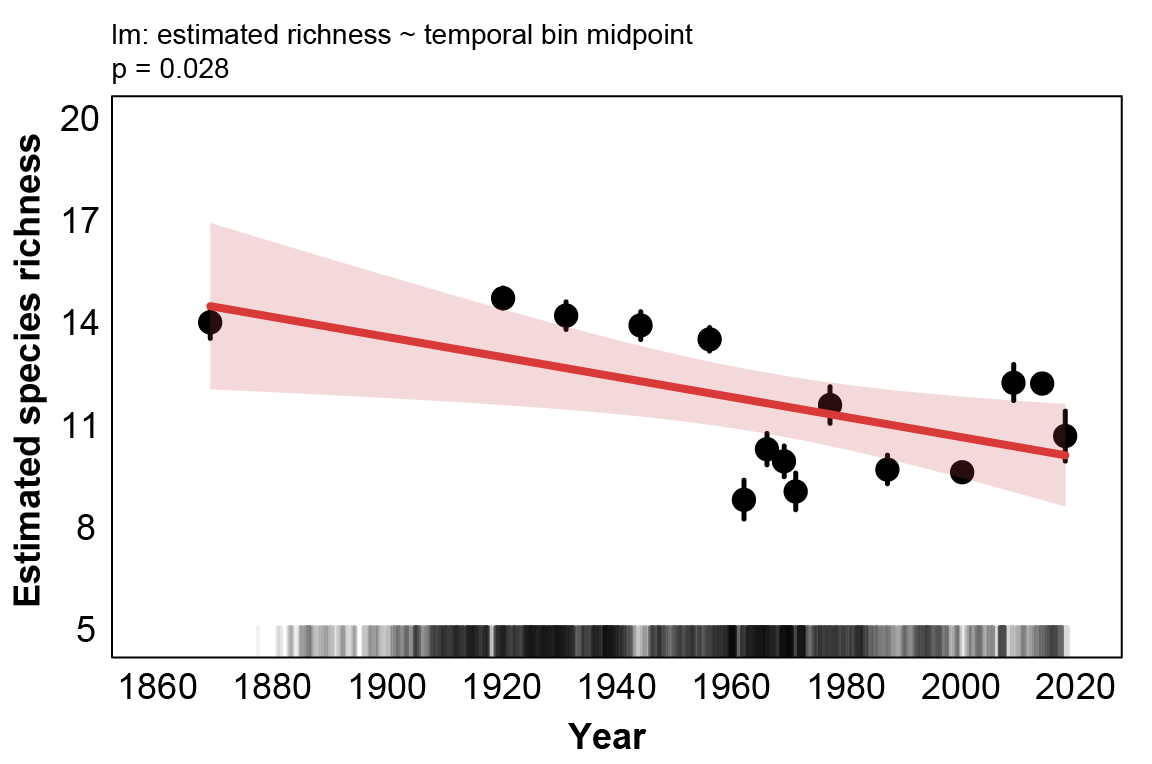
\includegraphics[width=0.6\textwidth,height=\textheight]{../ms_figs/fig1.png}

\textbf{Figure 1:} Trend in rarified bumble bee species richness from
1877-present. Each point represents a date range that is standardized to
contain an approximately equal number of bumble bee records (thus the
date range differs for each point), and it is plotted at the midpoint
year of the date range. Error bars are 95\% confidence intervals. The
fitted line is a linear model predicting estimated species richness as a
function of temporal bin order using the midpoint of the temporal bin as
the predictor. Carpet plot represents temporal collection year for all
records from 1877 to present.

\clearpage

\newpage

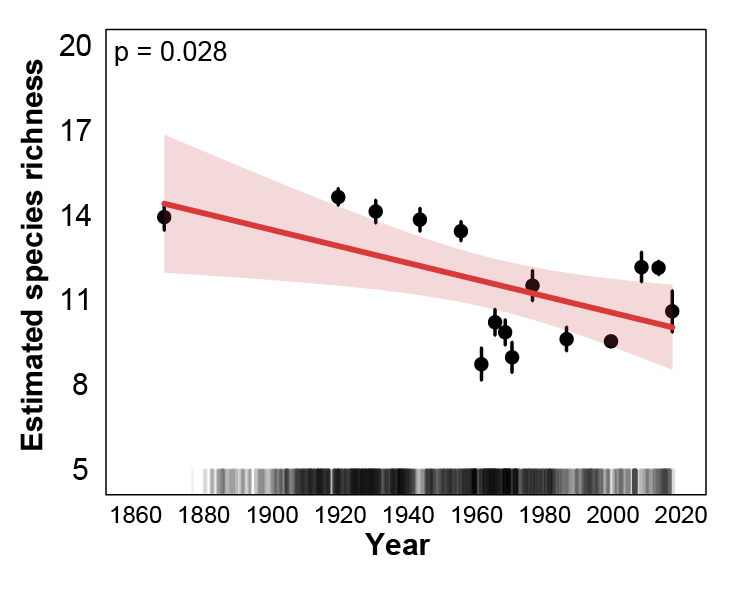
\includegraphics[width=1\textwidth,height=\textheight]{../ms_figs/fig2.png}

\textbf{Figure 2:} Patterns of agricultural intensification in two
metrics: (A) proportion of county under cultivation and (C) number of
crops grown per county. Inset graphs (B,D) depict general trend of these
variables for each state in the study area as modeled by a Loess curve.
Predicted probability of occurrence for two example species, \emph{B.
impatiens} (E,F) and \emph{B. terricola} (G,H) in each county given crop
diversity and proportion cropland in each county. Darker colors denote
smaller probability of occurrence, while lighter colors indicate larger
probability of occurrence. Red points on each map are randomly selected
occurrence records with a maximum of 50 plotted per year. (F,H) Fitted
temporal trend of relative abundance when modeled with agricultural
intensity metrics. Solid red lines denote statistically clear trend in
relative abundance over time (p \textless{} 0.05), while dashed lines
denote statistically unclear trends (p \textgreater{} 0.05). Points on
temporal trend are slightly jittered for visibility. Color palettes
derived using quantile binning. Values above maps are mean ± SEM for
each response.

\clearpage

\newpage

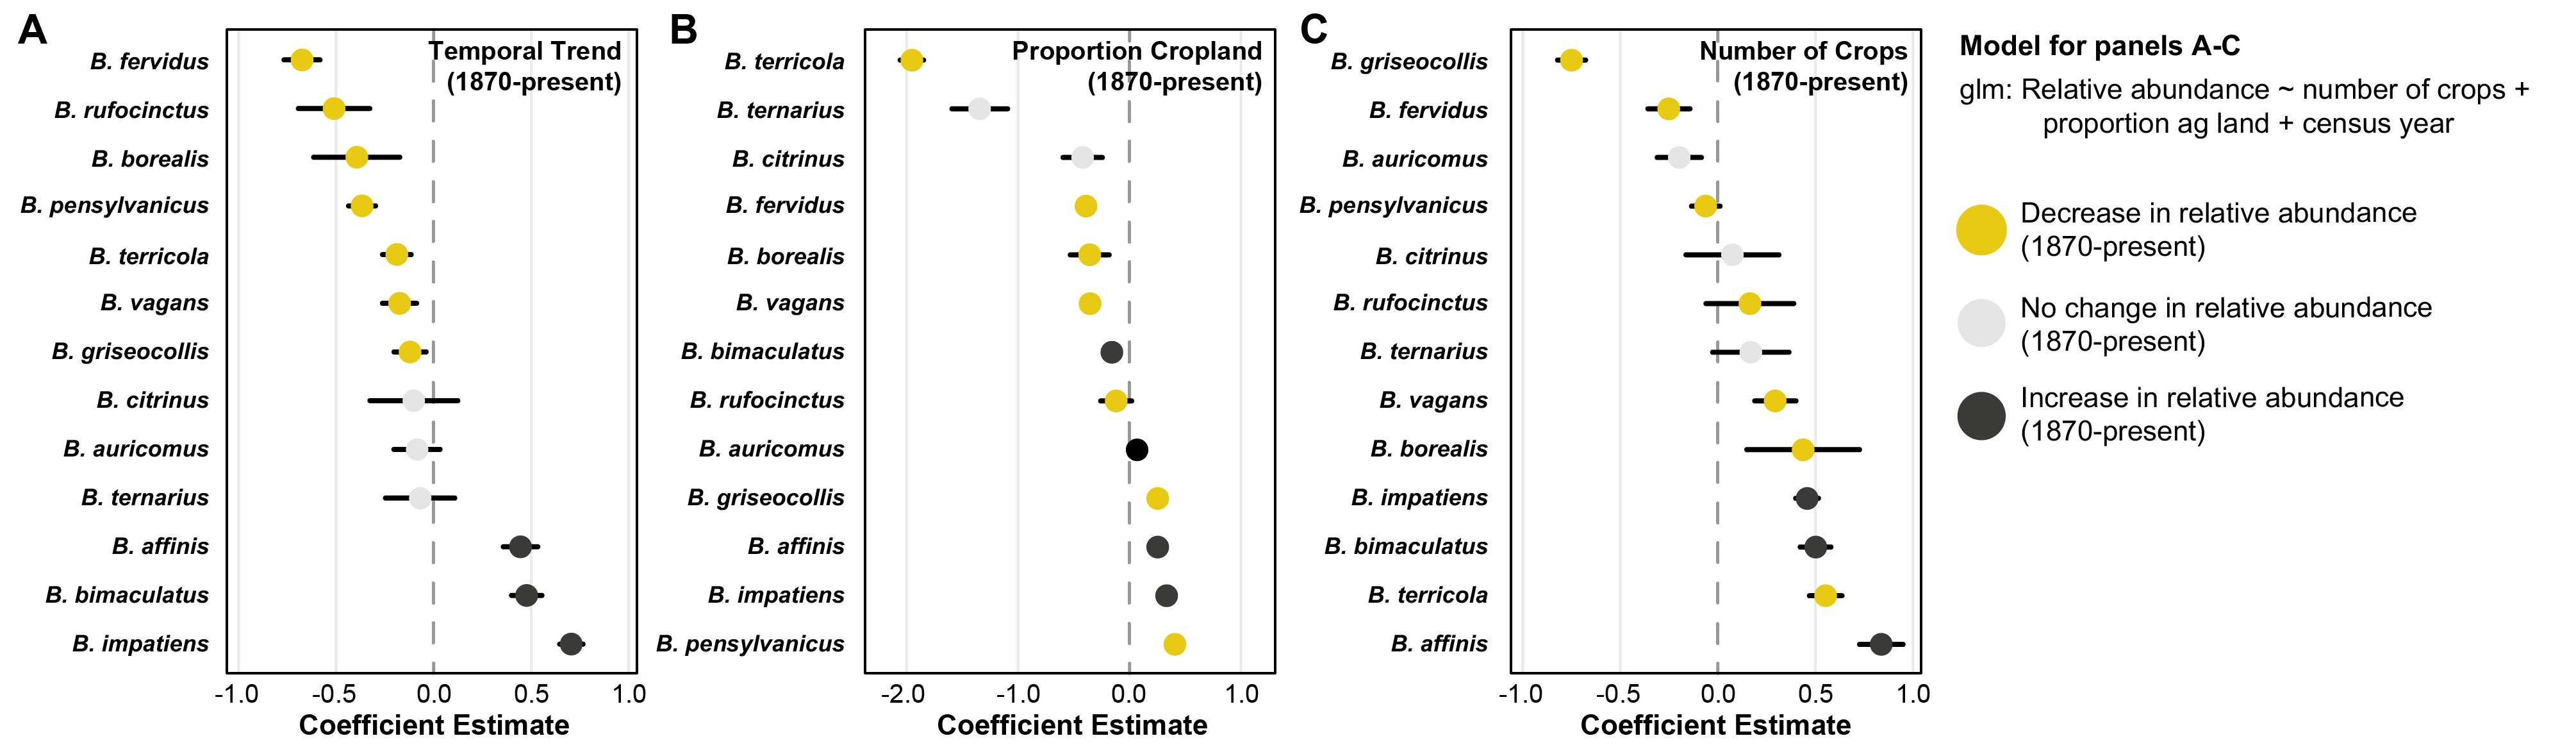
\includegraphics[width=1\textwidth,height=\textheight]{../ms_figs/fig3.png}

\textbf{Figure 3:} Fitted model coefficients (± 95\% confidence
interval) for the relative abundance of each study species for (A)
temporal trend of the species, (B) proportion of county in cropland, and
(C) the number of crops grown in a county. Models were fitted using the
entire dataset from 1870-present. The relative abundance trend from
1870-present (a) denotes point colors for b \& c: yellow points are
species whose relative abundance declined, gray points are no change in
relative abundance, and black points denote increases in relative
abundance.

\clearpage

\newpage

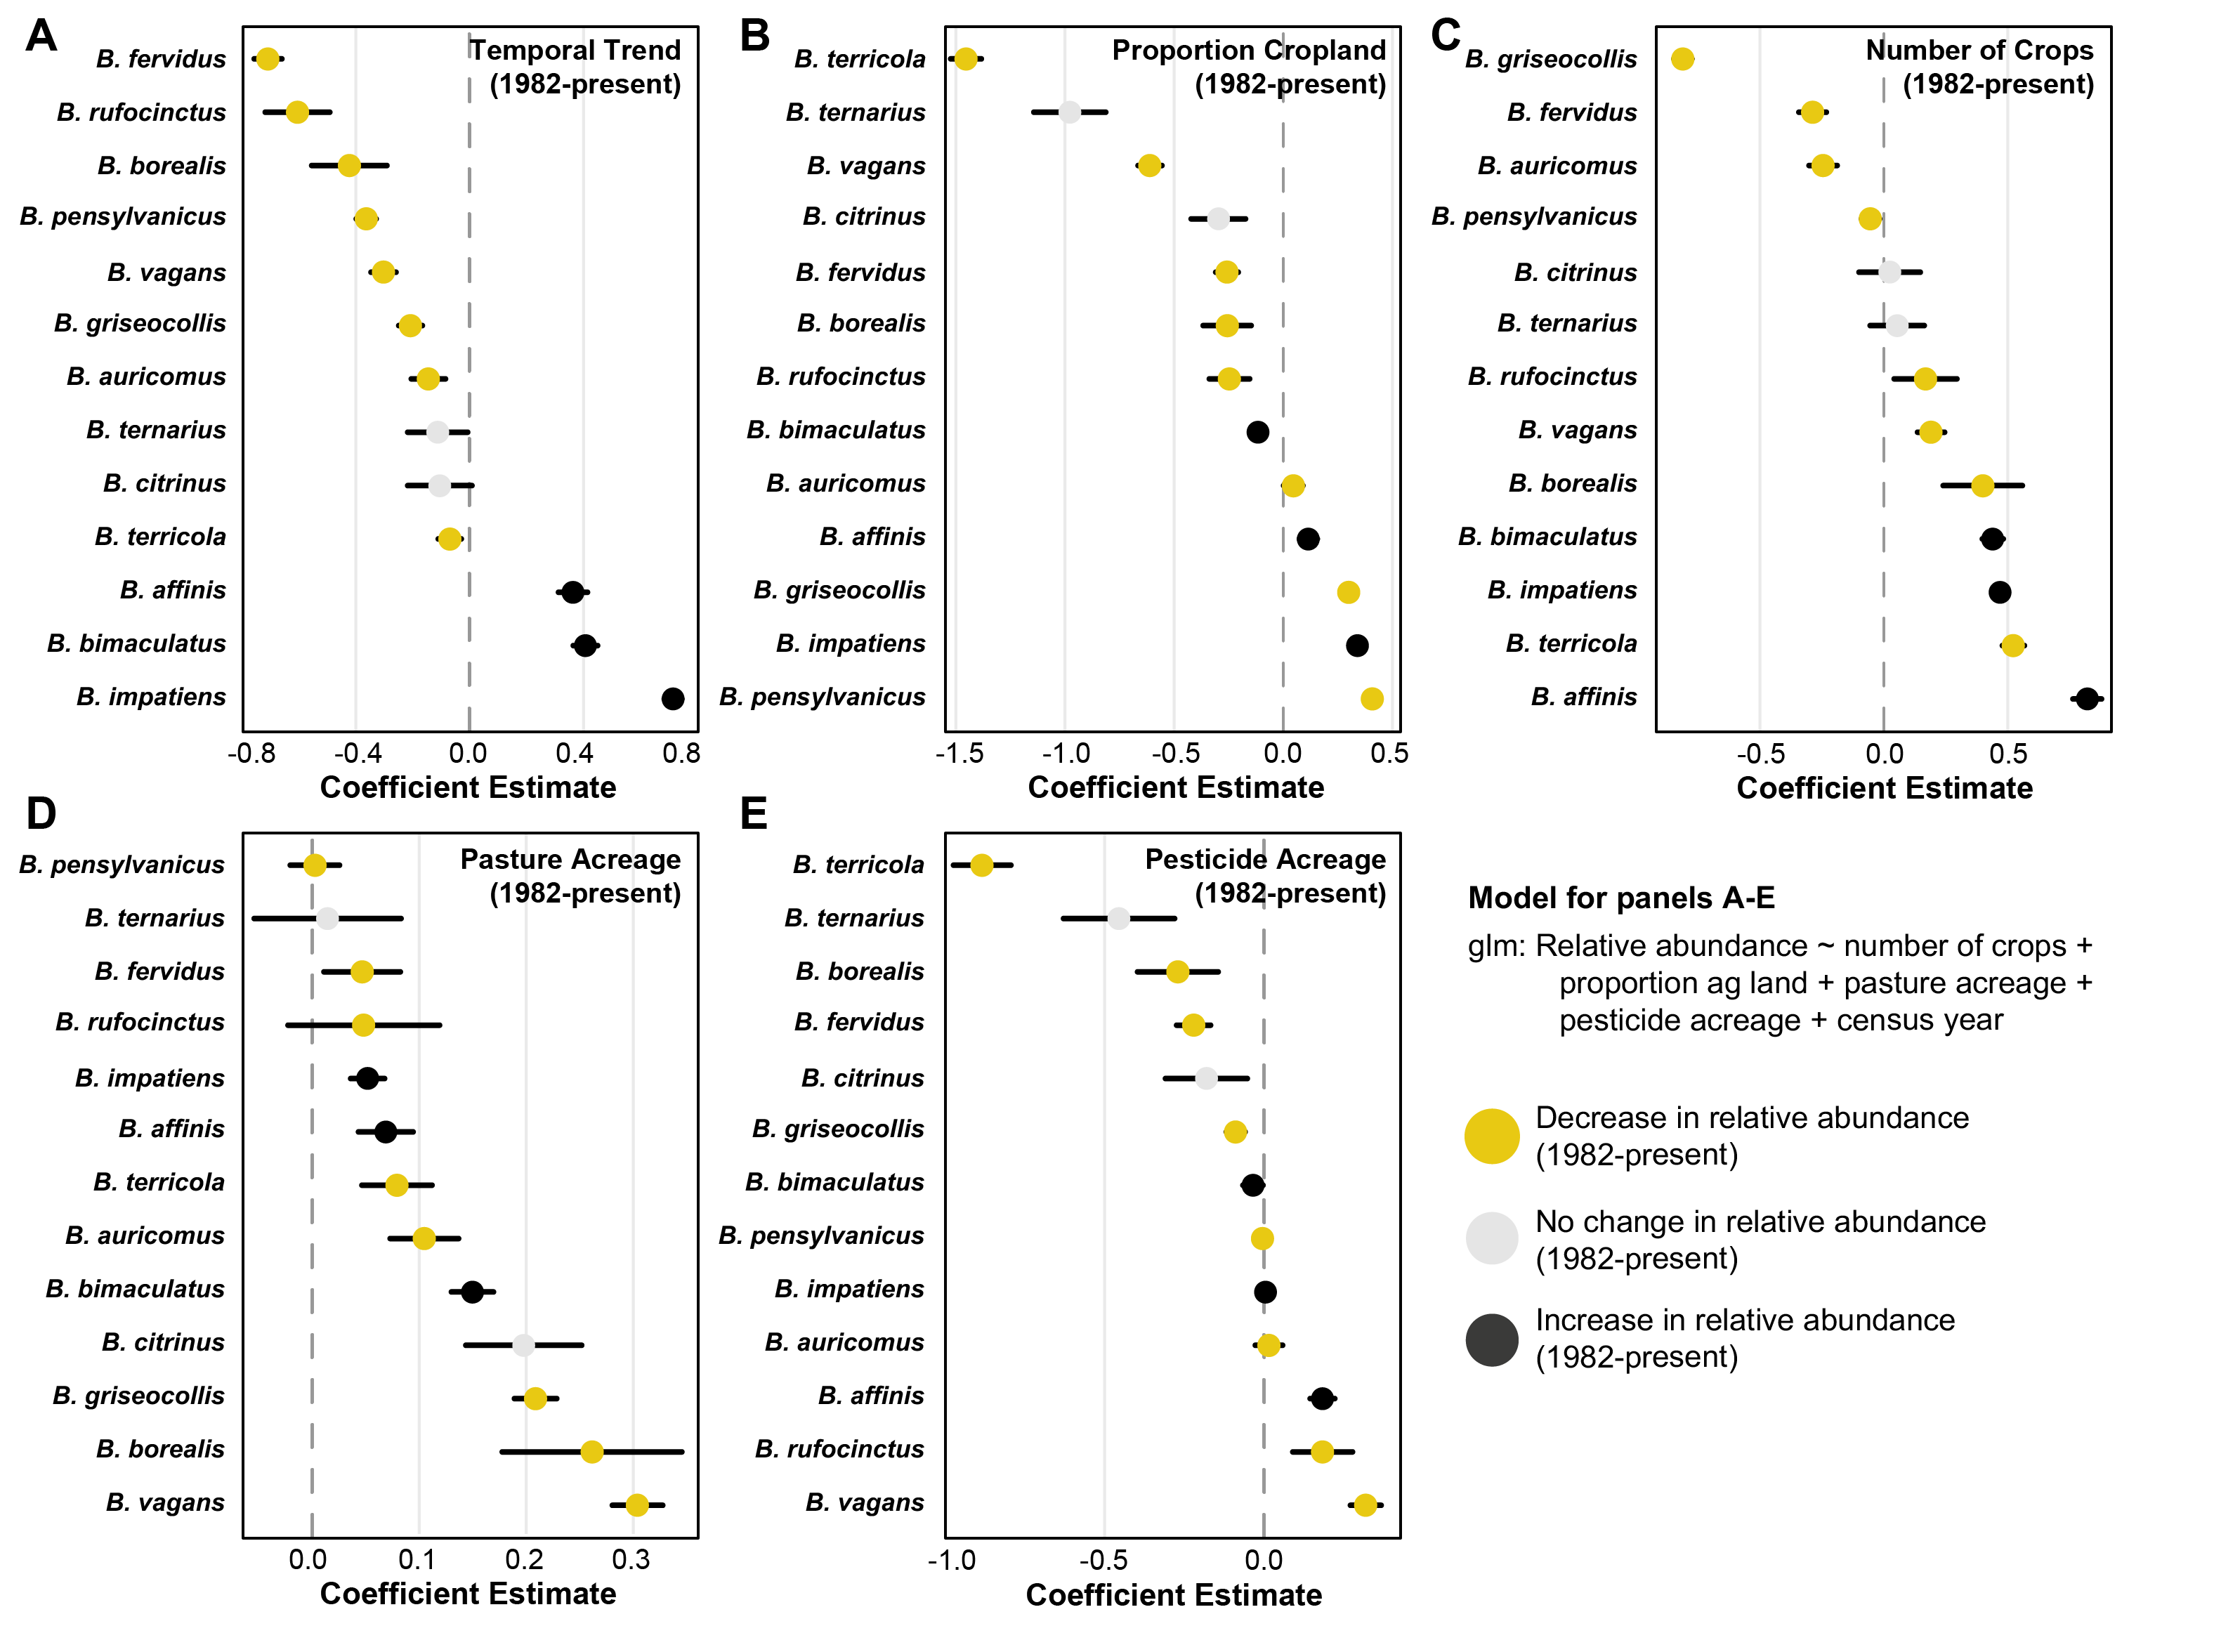
\includegraphics[width=1\textwidth,height=\textheight]{../ms_figs/fig5.png}

\textbf{Figure 4:} Fitted model coefficients (± 95\% confidence
interval) for each study species for (A) temporal trend of the species,
(B) proportion of county in cropland, and (C) the number of crops grown
in a county, (D) acres of pasture grown in a county, and (E) acres
treated with insecticides. Models were fitted using data from
1982-present (only years for which pesticide and pasture acreage are
available across all counties). Point colors indicate species relative
abundance trend from 1982-present: yellow points denote species whose
relative abundance declined, gray points denote no change in relative
abundance, and black points denote increases in relative abundance.

\clearpage

\newpage

\hypertarget{supplementary-material}{%
\section{Supplementary Material}\label{supplementary-material}}

\hypertarget{appendix-1}{%
\subsubsection{Appendix 1}\label{appendix-1}}

\textbf{Analysis filtering data to unique \emph{species x location x
collector x date} combinations}

To determine whether sampling effort by individuals skewed the results
of our analysis, we fit our primary model
(\texttt{relative\ abundance\ \textasciitilde{}\ proportion\ cropland\ +\ number\ of\ crops\ +\ agricultural\ census\ year};
results shown in Fig. 3) to a reduced dataset, filtering records to
include only unique combinations of species, location, collector, and
collection date. We found similar results in terms of the effect
magnitude of predictors (proportion of cropland and number of crops), as
well as the direction of the effect across study species (Fig. SA1.1).

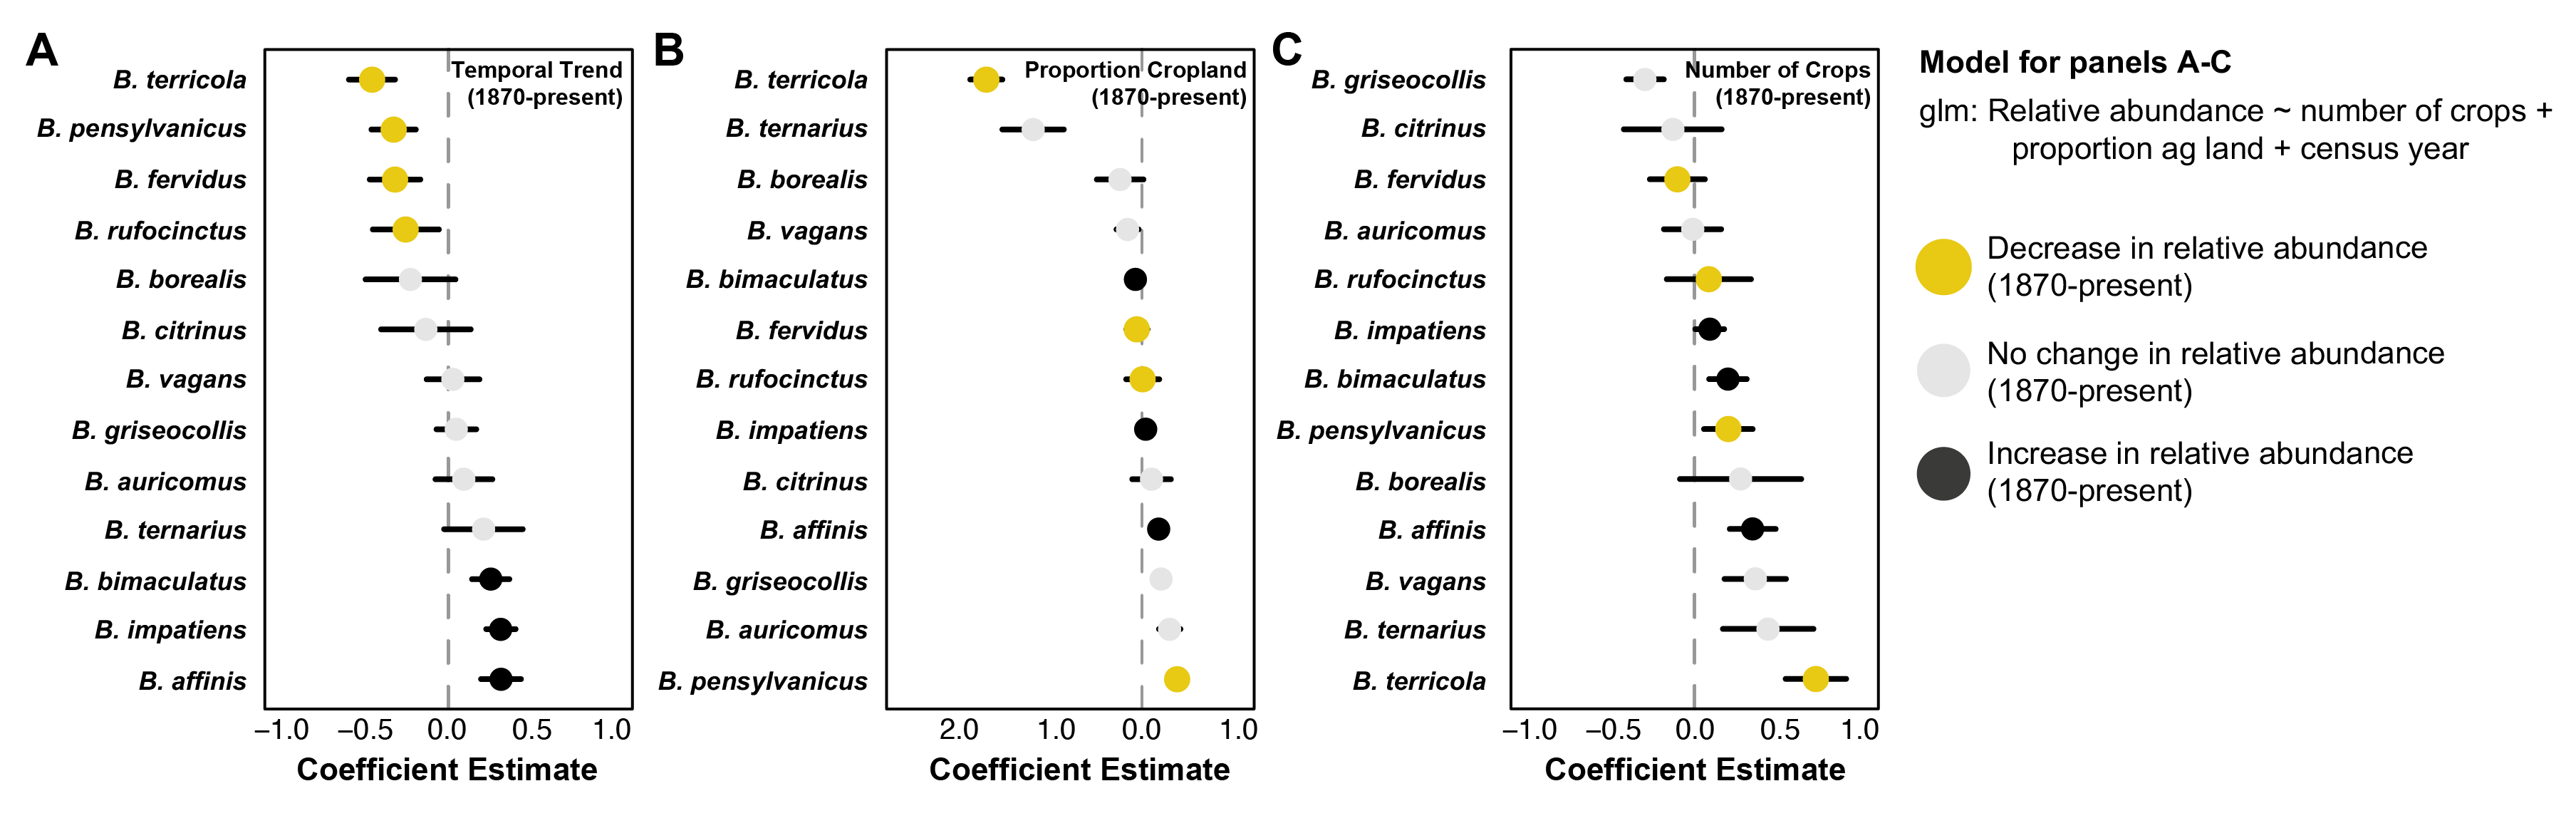
\includegraphics[width=1\textwidth,height=\textheight]{../ms_figs/appendix1.png}
\textbf{Figure SA1.1} Fitted model coefficients (± 95\% confidence
interval) for each study species for (A) temporal trend of the species,
(B) proportion of county in cropland, and (C) the number of crops grown
in a county. Models were fitted using the entire dataset from
1870-present, but filtered to unique species x location x collector x
date combinations. Point colors indicate species relative abundance
trend from 1870-present: yellow points denote species whose relative
abundance declined, gray points denote no change in relative abundance,
and black points denote increases in relative abundance.

\clearpage

\newpage

\hypertarget{appendix-2}{%
\subsubsection{Appendix 2}\label{appendix-2}}

\textbf{Analysis restricting to records within ± 2 years of agricultural
census}

As agricultural census records are collected every 10 years, we were
required to pair bumble bee records to the nearest agricultural census
(a difference of up to ± 5 years). This requirement might skew results
if agricultural metrics display non-linear trends between census years.
TO determine if this was the case, we filtered records such that only
bumble bee within ± 2 years of an agricultural census data were
included. Modeling these data resulted in broadly similar patterns of
species relative abundance trends and response to proportion
agriculture. The response of species to number of crops showed the
effect magnitude increase for some species, but the rank order of
species responses was mostly similar (Fig. SA2.1).

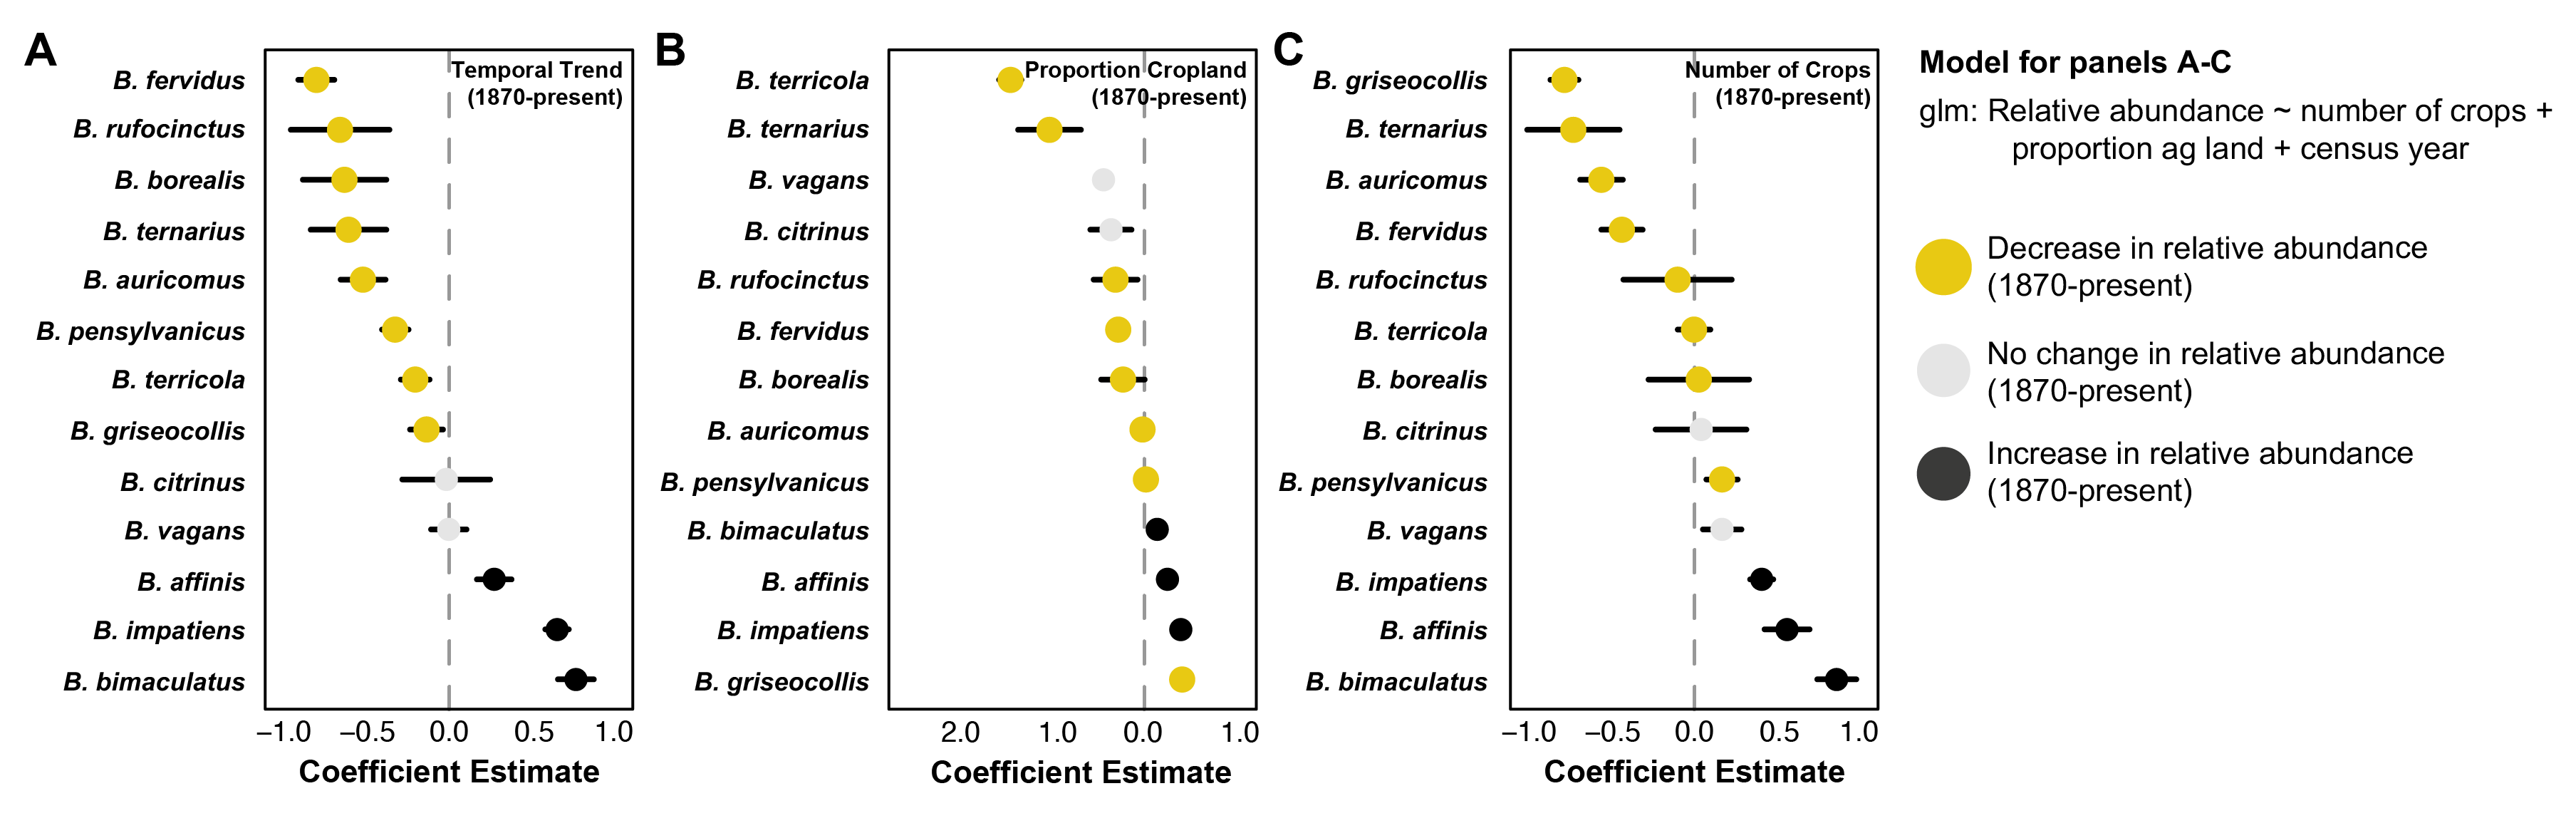
\includegraphics[width=1\textwidth,height=\textheight]{../ms_figs/appendix2.png}
\textbf{Figure SA1.1} Fitted model coefficients (± 95\% confidence
interval) for each study species for (A) temporal trend of the species,
(B) proportion of county in cropland, and (C) the number of crops grown
in a county. Models were fitted using the entire dataset from
1870-present, but filtered to only include bumble bee records within ± 2
years of an agricultural census. Point colors indicate species relative
abundance trend from 1870-present: yellow points denote species whose
relative abundance declined, gray points denote no change in relative
abundance, and black points denote increases in relative abundance.

\newpage

\hypertarget{appendix-3}{%
\subsubsection{Appendix 3}\label{appendix-3}}

\textbf{Raw changes in species relative abundance over time}

For each species, we calculated relative abundance for each temporal bin
as the number of records of a given species divided by the total number
of records for all species in that temporal bin. We then tested whether
there was a statistically clear change in relative abundance over time
by fitting generalized linear models with binomial error distributions
for each species using time (i.e., temporal bin) as the sole predictor
with each point weighted by the number of records (similar to Bartomeus
et al. 2013).

Of the 13 species included in our simple analysis of change in relative
abundance over time, 6 saw statistically clear reductions in relative
abundance: \emph{B. borealis}, \emph{B. fervidus}, \emph{B.
pensylvanicus}, \emph{B. rufocinctus}, \emph{B. terricola}, \emph{B.
vagans} (Table S1). Similar to the patterns of estimated species
richness, reductions in the relative abundance of these declining
species seem to begin in the middle of the 20th century. There were 7
species which increased in relative abundance over time period covered
by this dataset: \emph{B. affinis}, \emph{B. auricomus}, \emph{B.
bimaculatus}, \emph{B. citrinus}, \emph{B. griseocollis}, \emph{B.
impatiens}, and \emph{B. ternarius}.

\textbf{Table SA3.1:} Relative abundance estimates for each species
across 8 time bins, sized in order to contain approximately equal
numbers of bumble bee records per bin. Coefficient estimates and
p-values derived from models fit to estimate trends in relative
abundance over time, where relative abundance of each species is
predicted by time bin fit using a generalized linear model, with N
records representing the number of records for a given species.

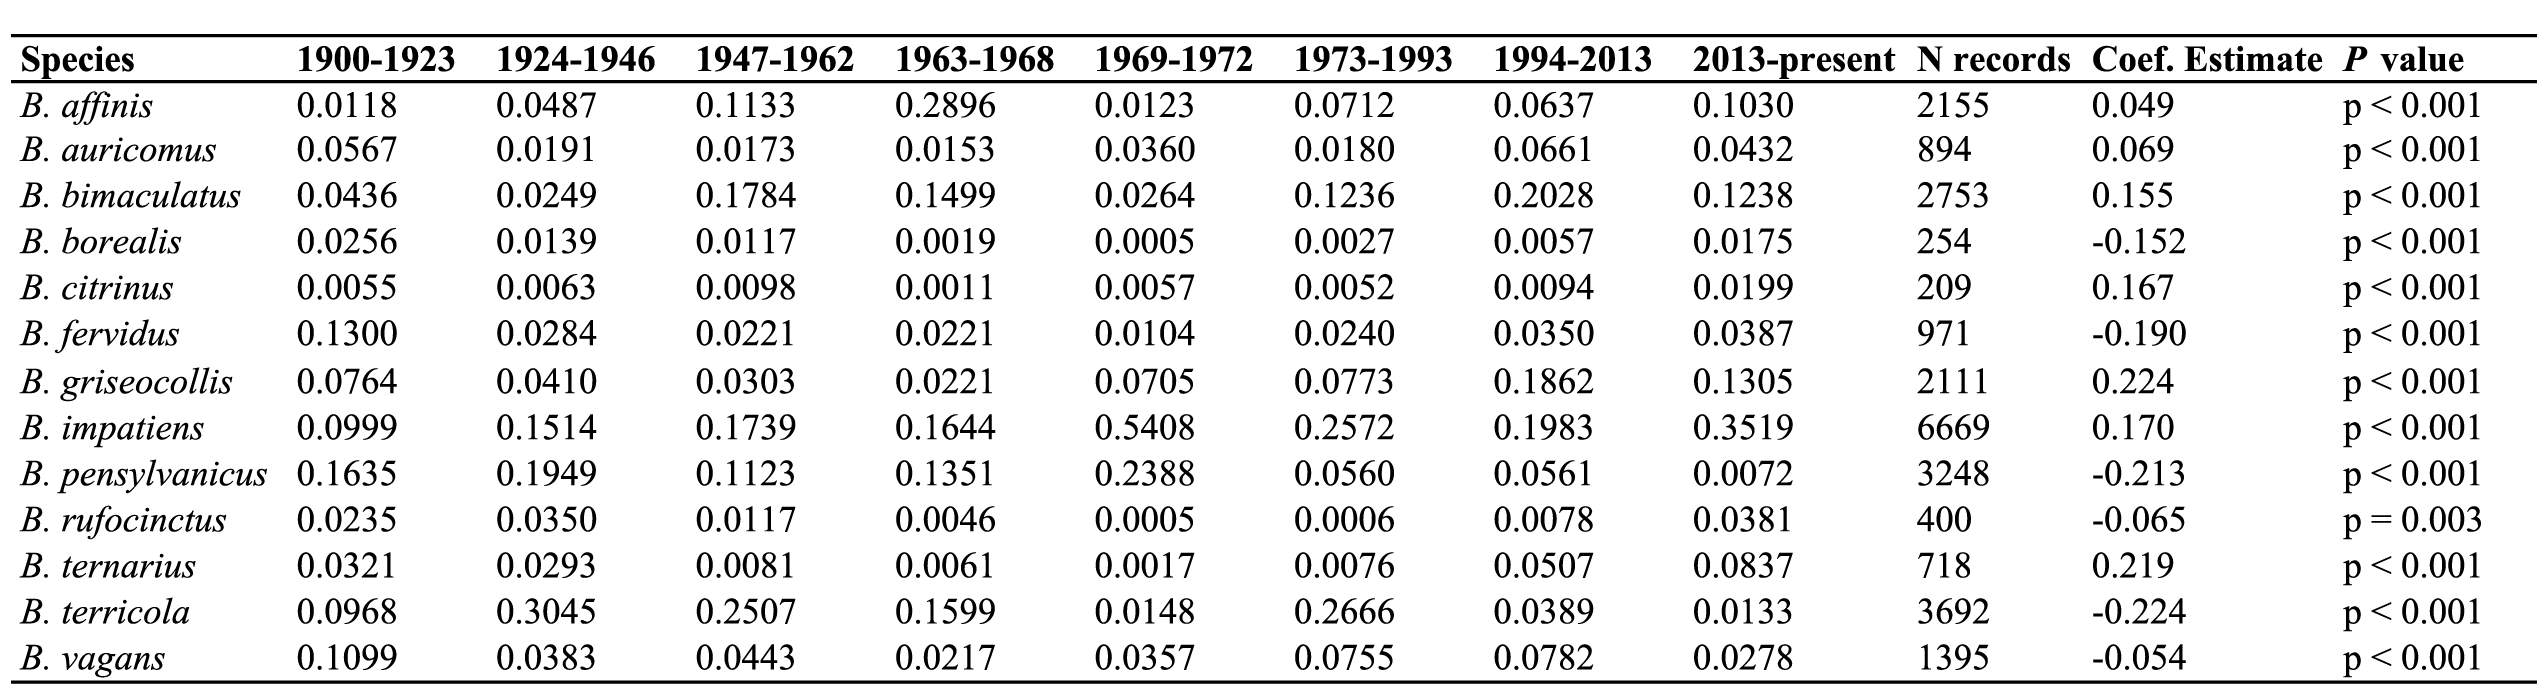
\includegraphics[width=1\textwidth,height=\textheight]{../ms_figs/table1.png}

\clearpage

\textbf{Supplementary Table 1:} Generalized linear model results for
each study species including the sample size (number of counties for
which relative abundance is calculated), model term, scaled coefficient
estimate, 95\% confidence interval and p-value. Each county is weighted
by the total number of bumble bee records for a given time point
(agricultural census year).

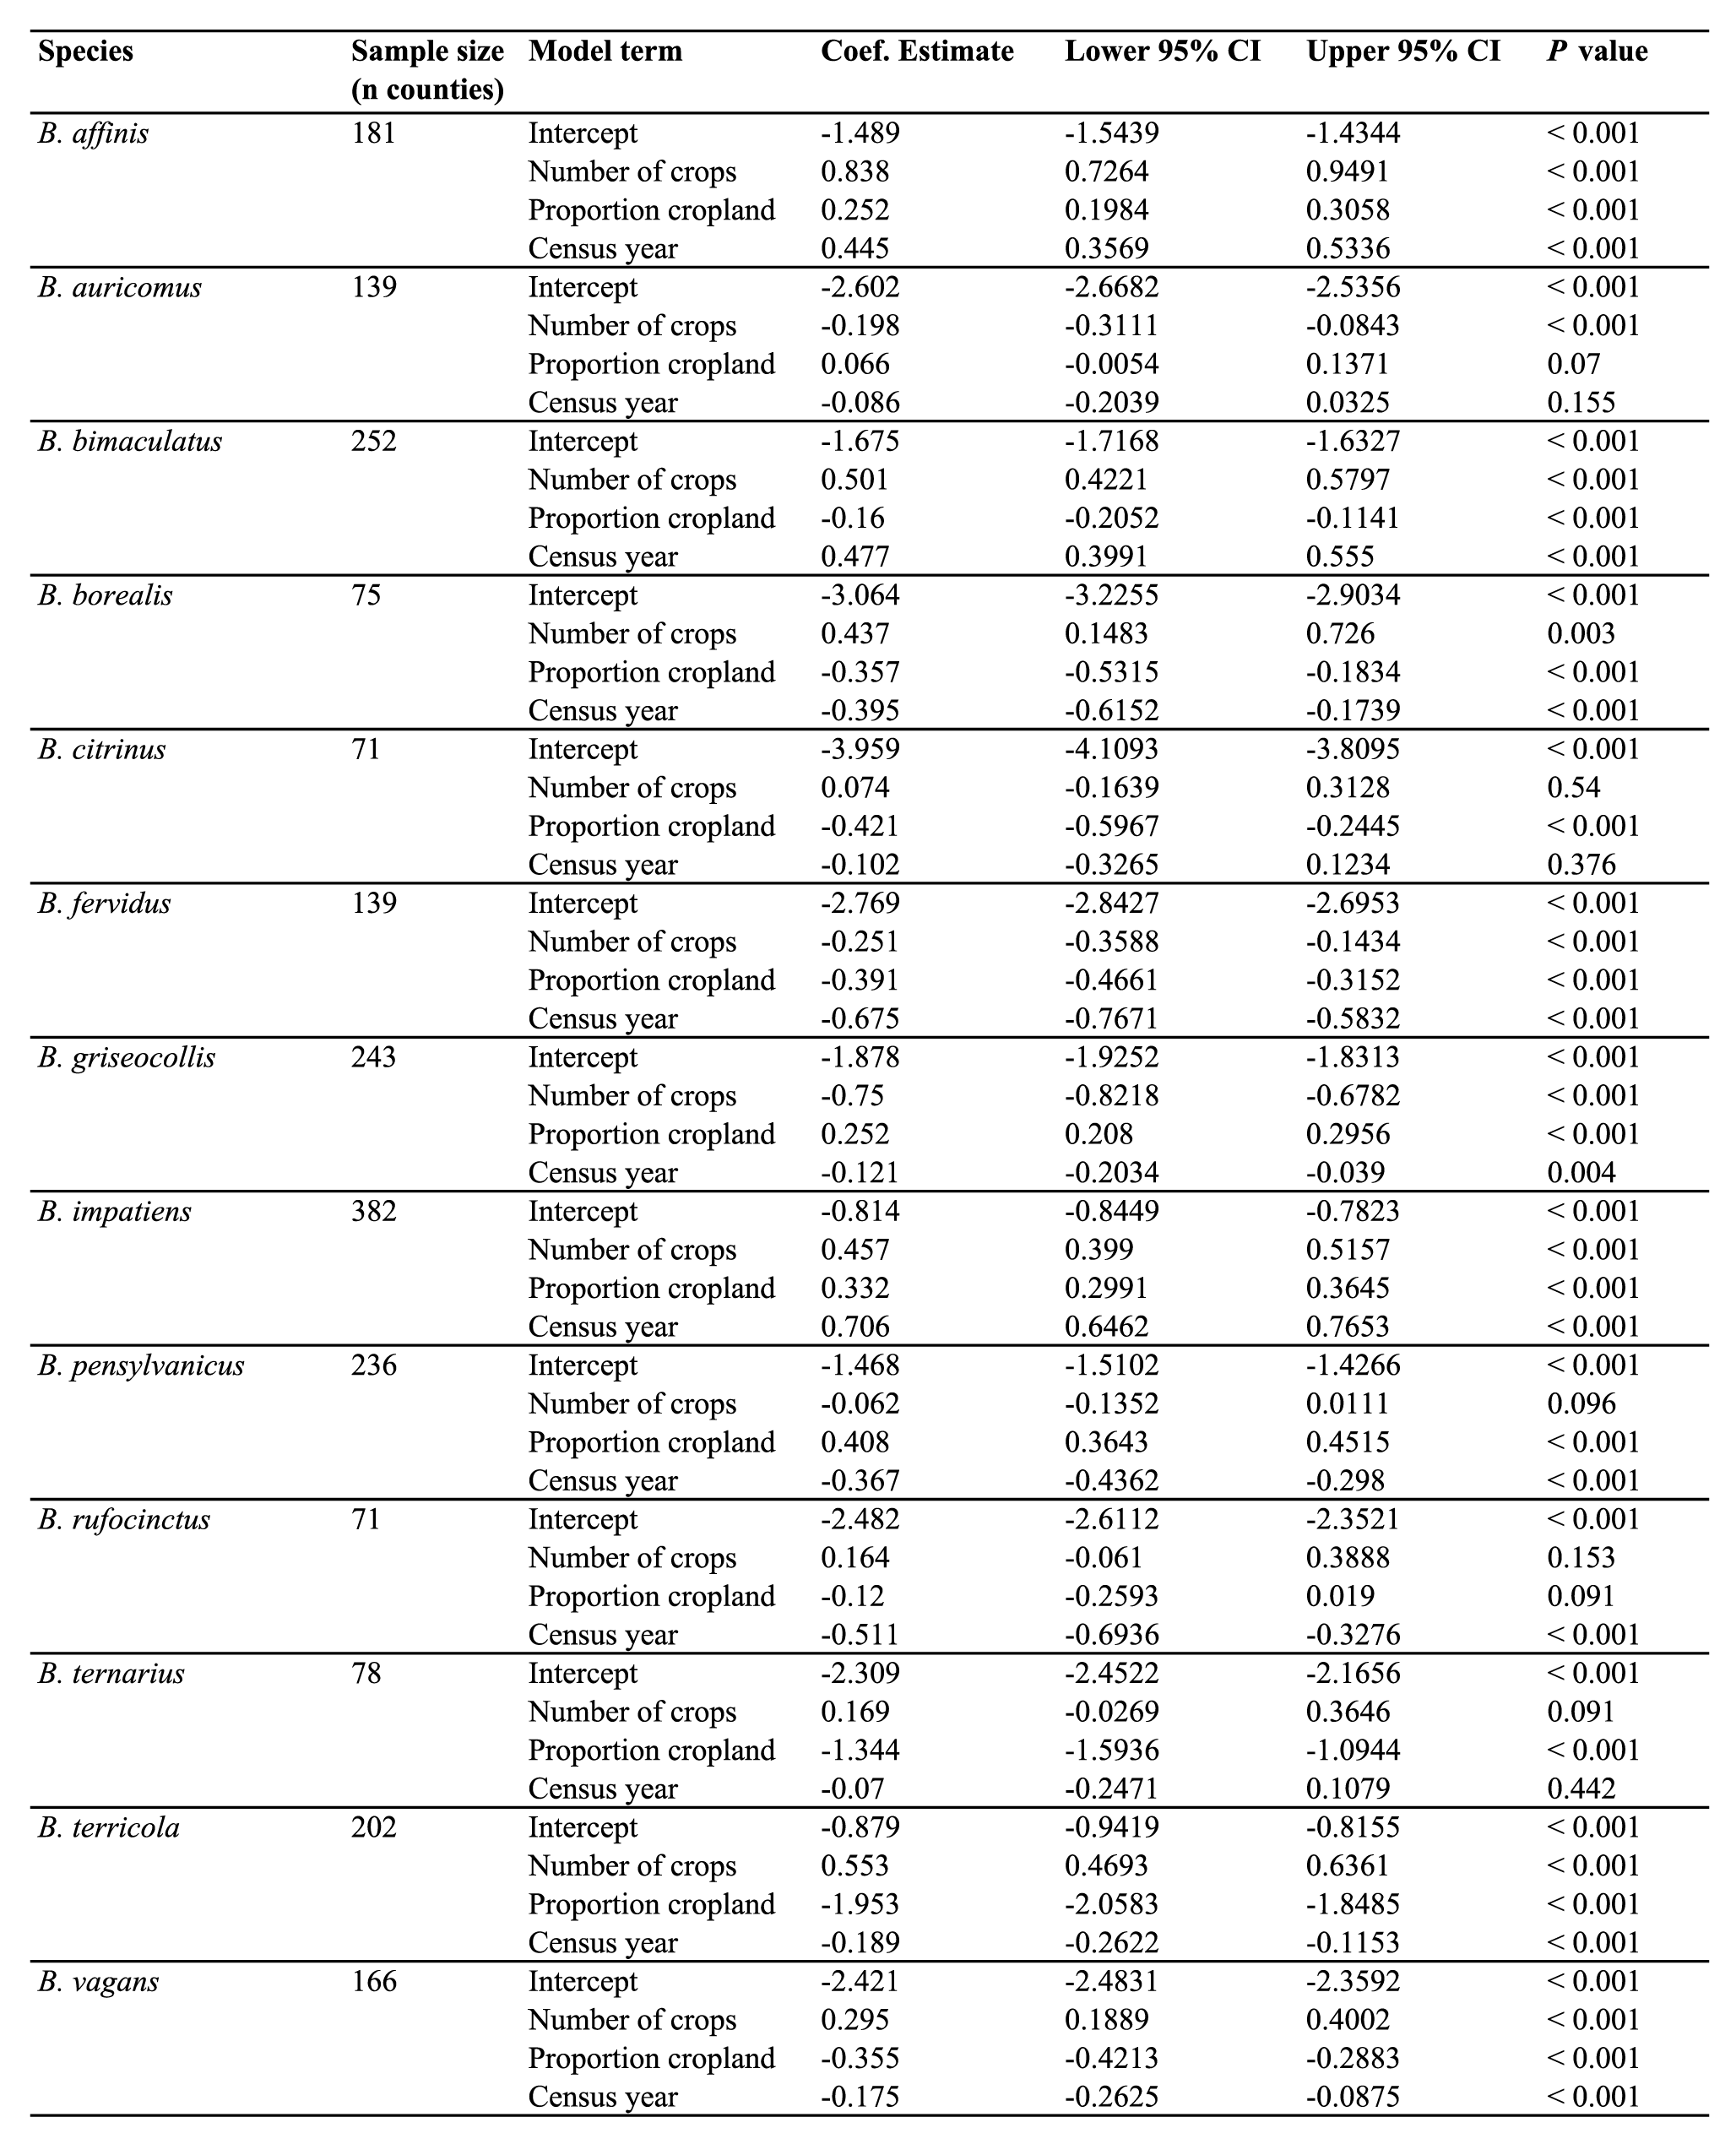
\includegraphics[width=0.6\textwidth,height=\textheight]{../ms_figs/tables1.png}

\clearpage

\textbf{Supplementary Table 3:} Generalized linear model results for
each study species including the sample size (number of counties for
which relative abundance is calculated), model term, scaled coefficient
estimate, 95\% confidence interval and p-value. Each county is weighted
by the total number of bumble bee records for a given time point
(agricultural census year).

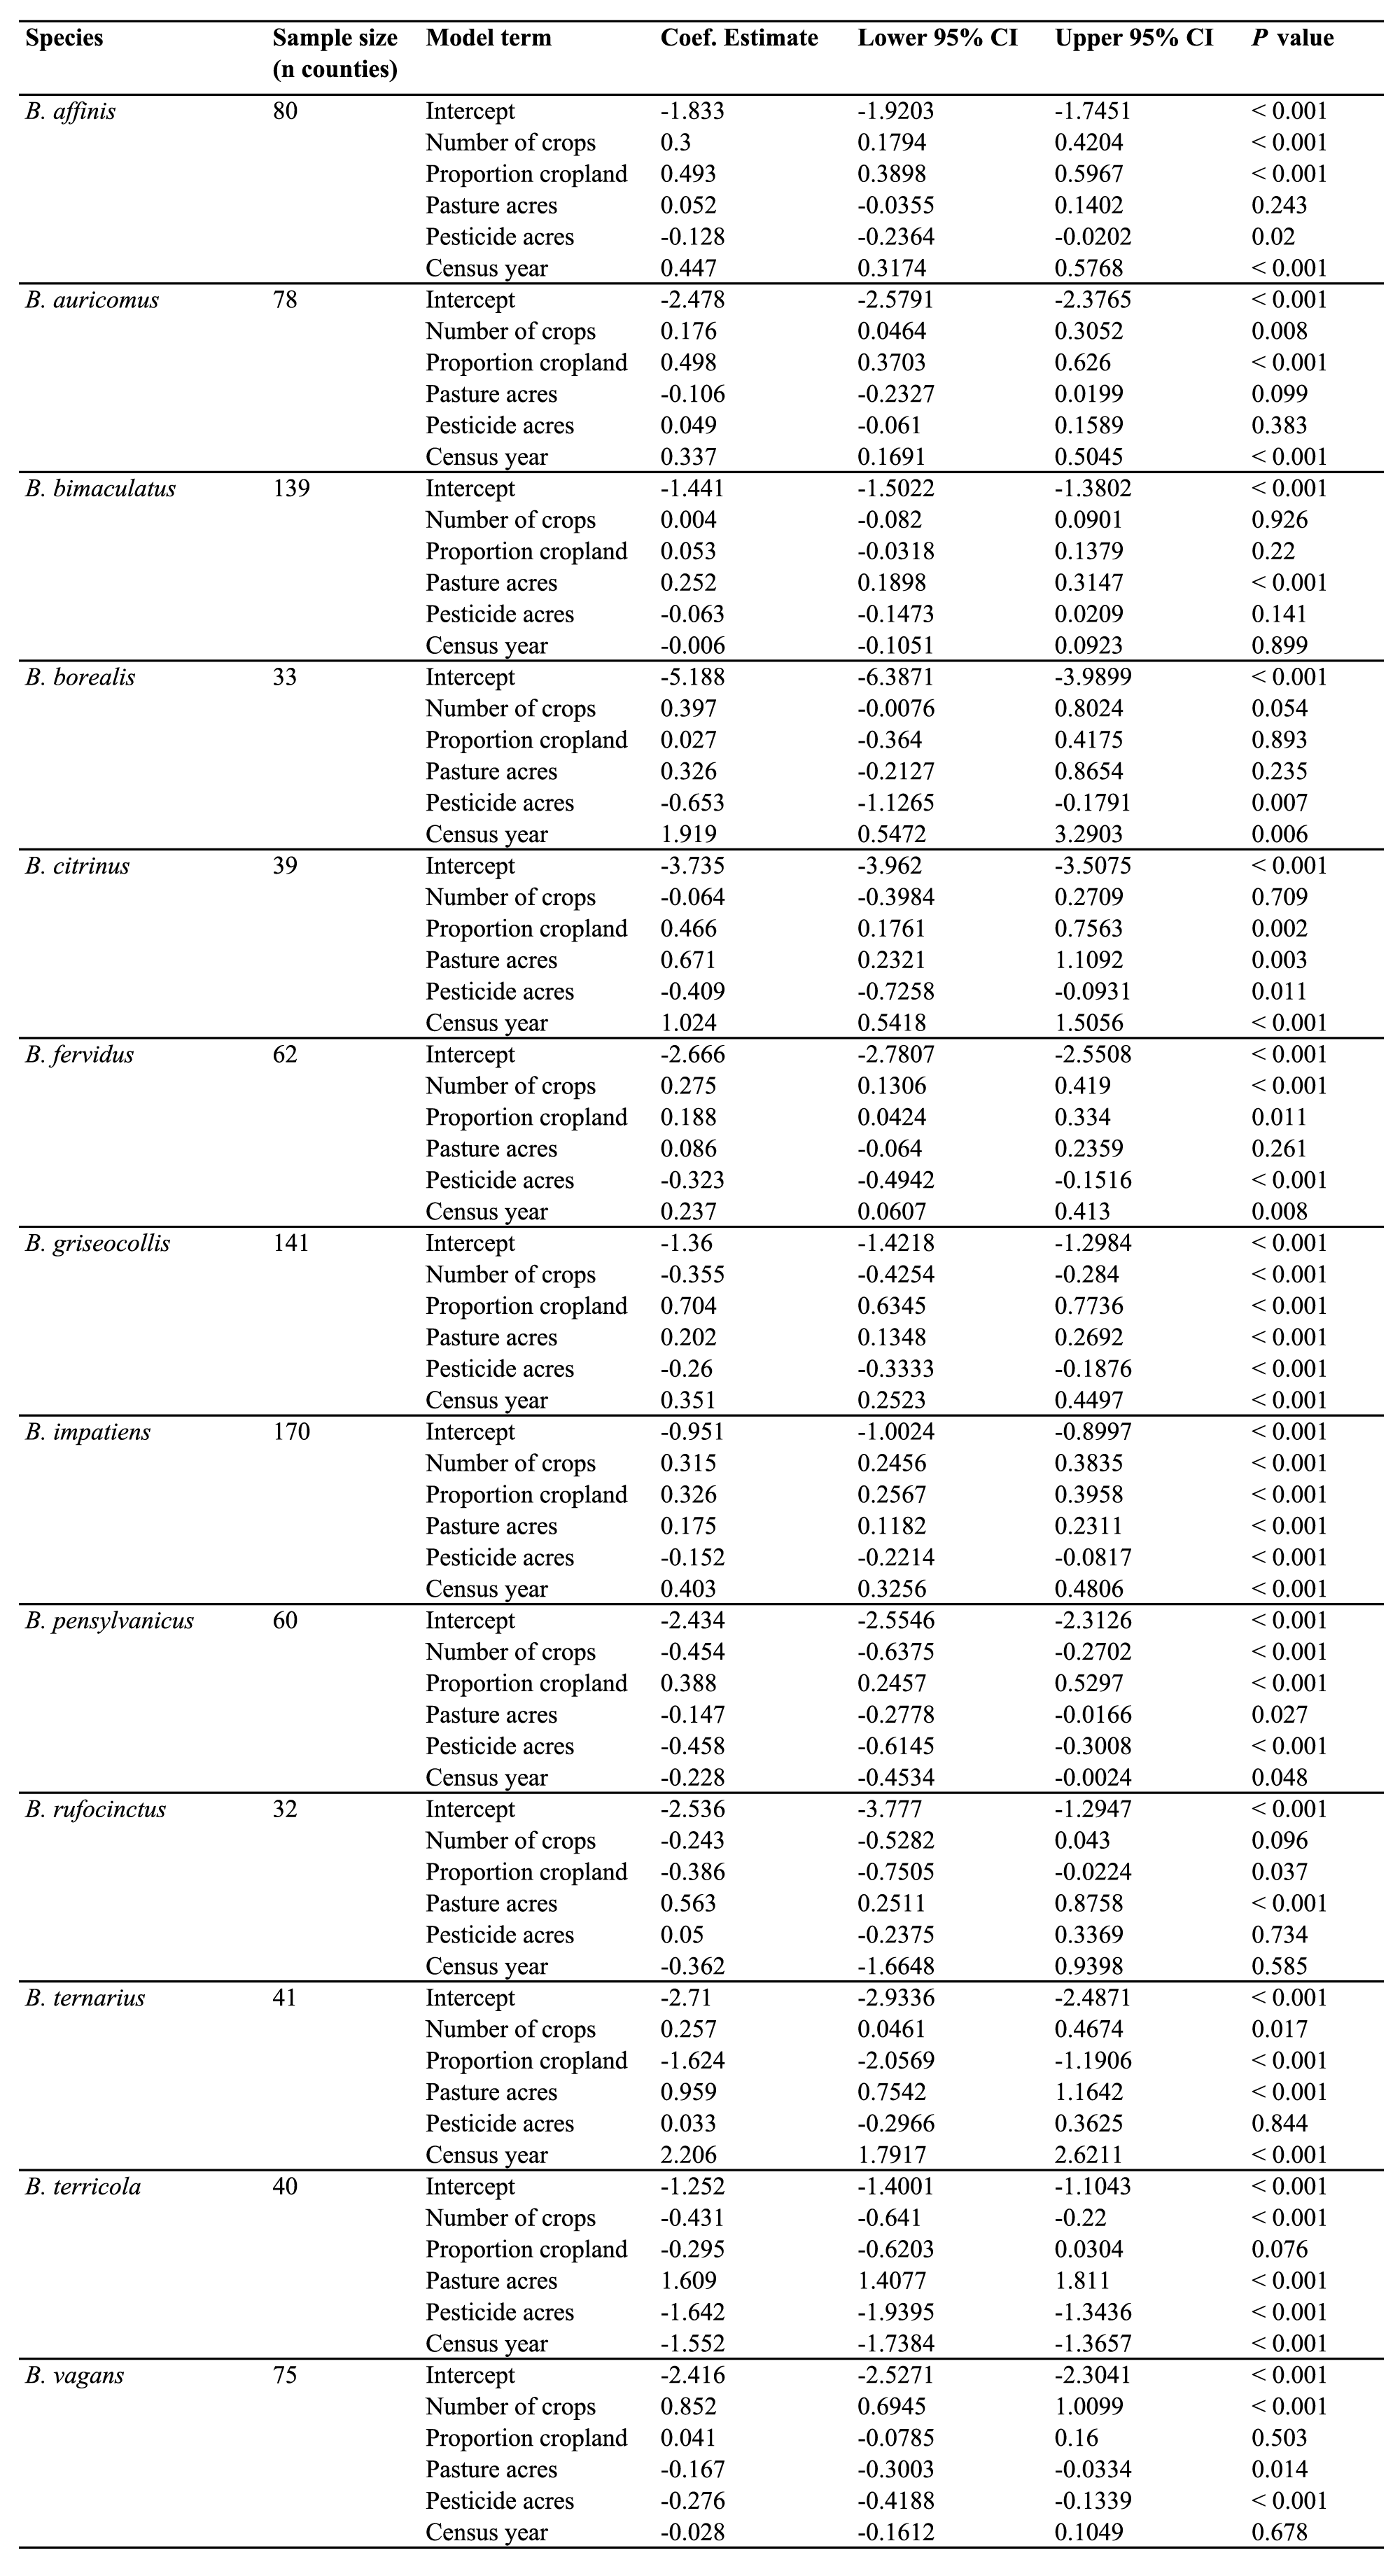
\includegraphics[width=0.6\textwidth,height=\textheight]{../ms_figs/tables2.png}

\clearpage

\newpage

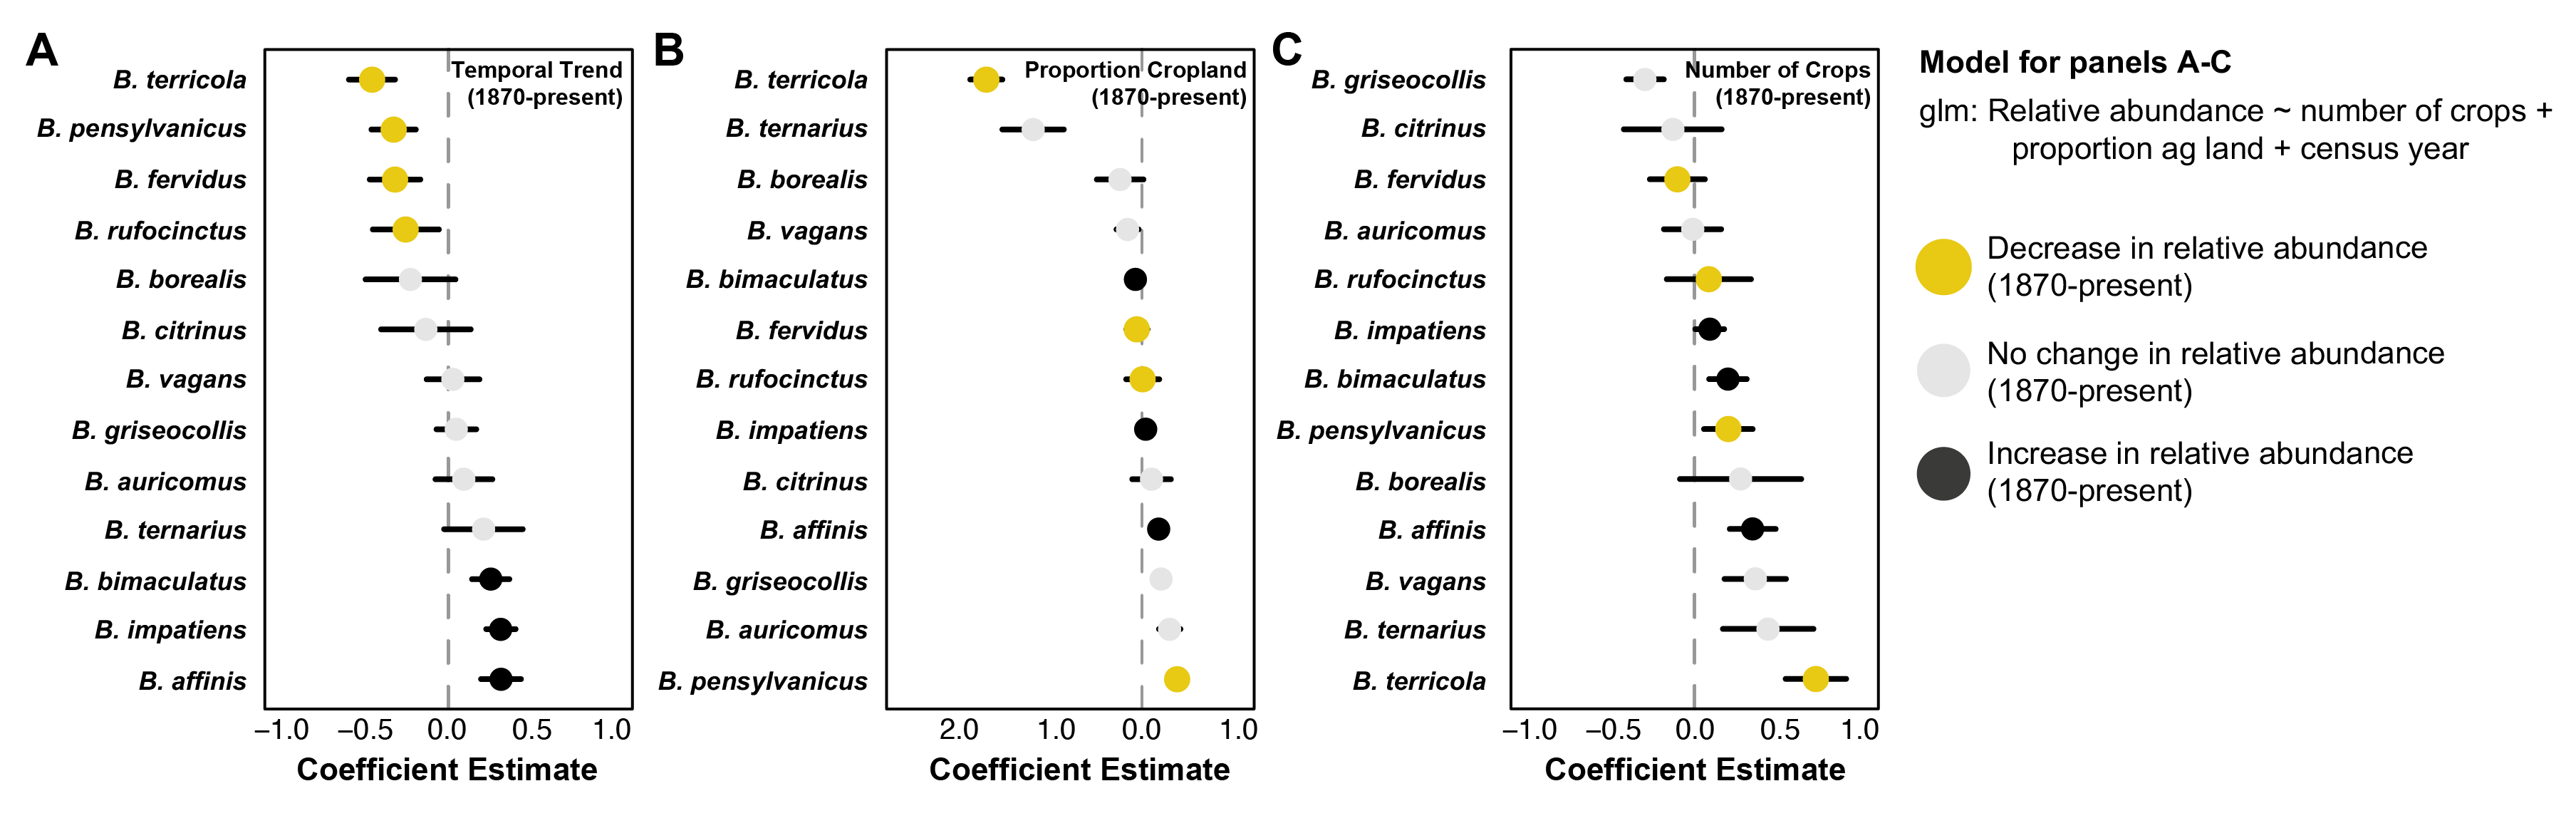
\includegraphics[width=0.8\textwidth,height=\textheight]{../ms_figs/fig_s2.png}

\textbf{Supplementary Figure 1:} The location of bumble bee records for
each US Census of Agriculture year considered in our analysis. The
number of records is noted below the year. Points are partially
transparent and jittered slightly for visibility.

\clearpage

\newpage

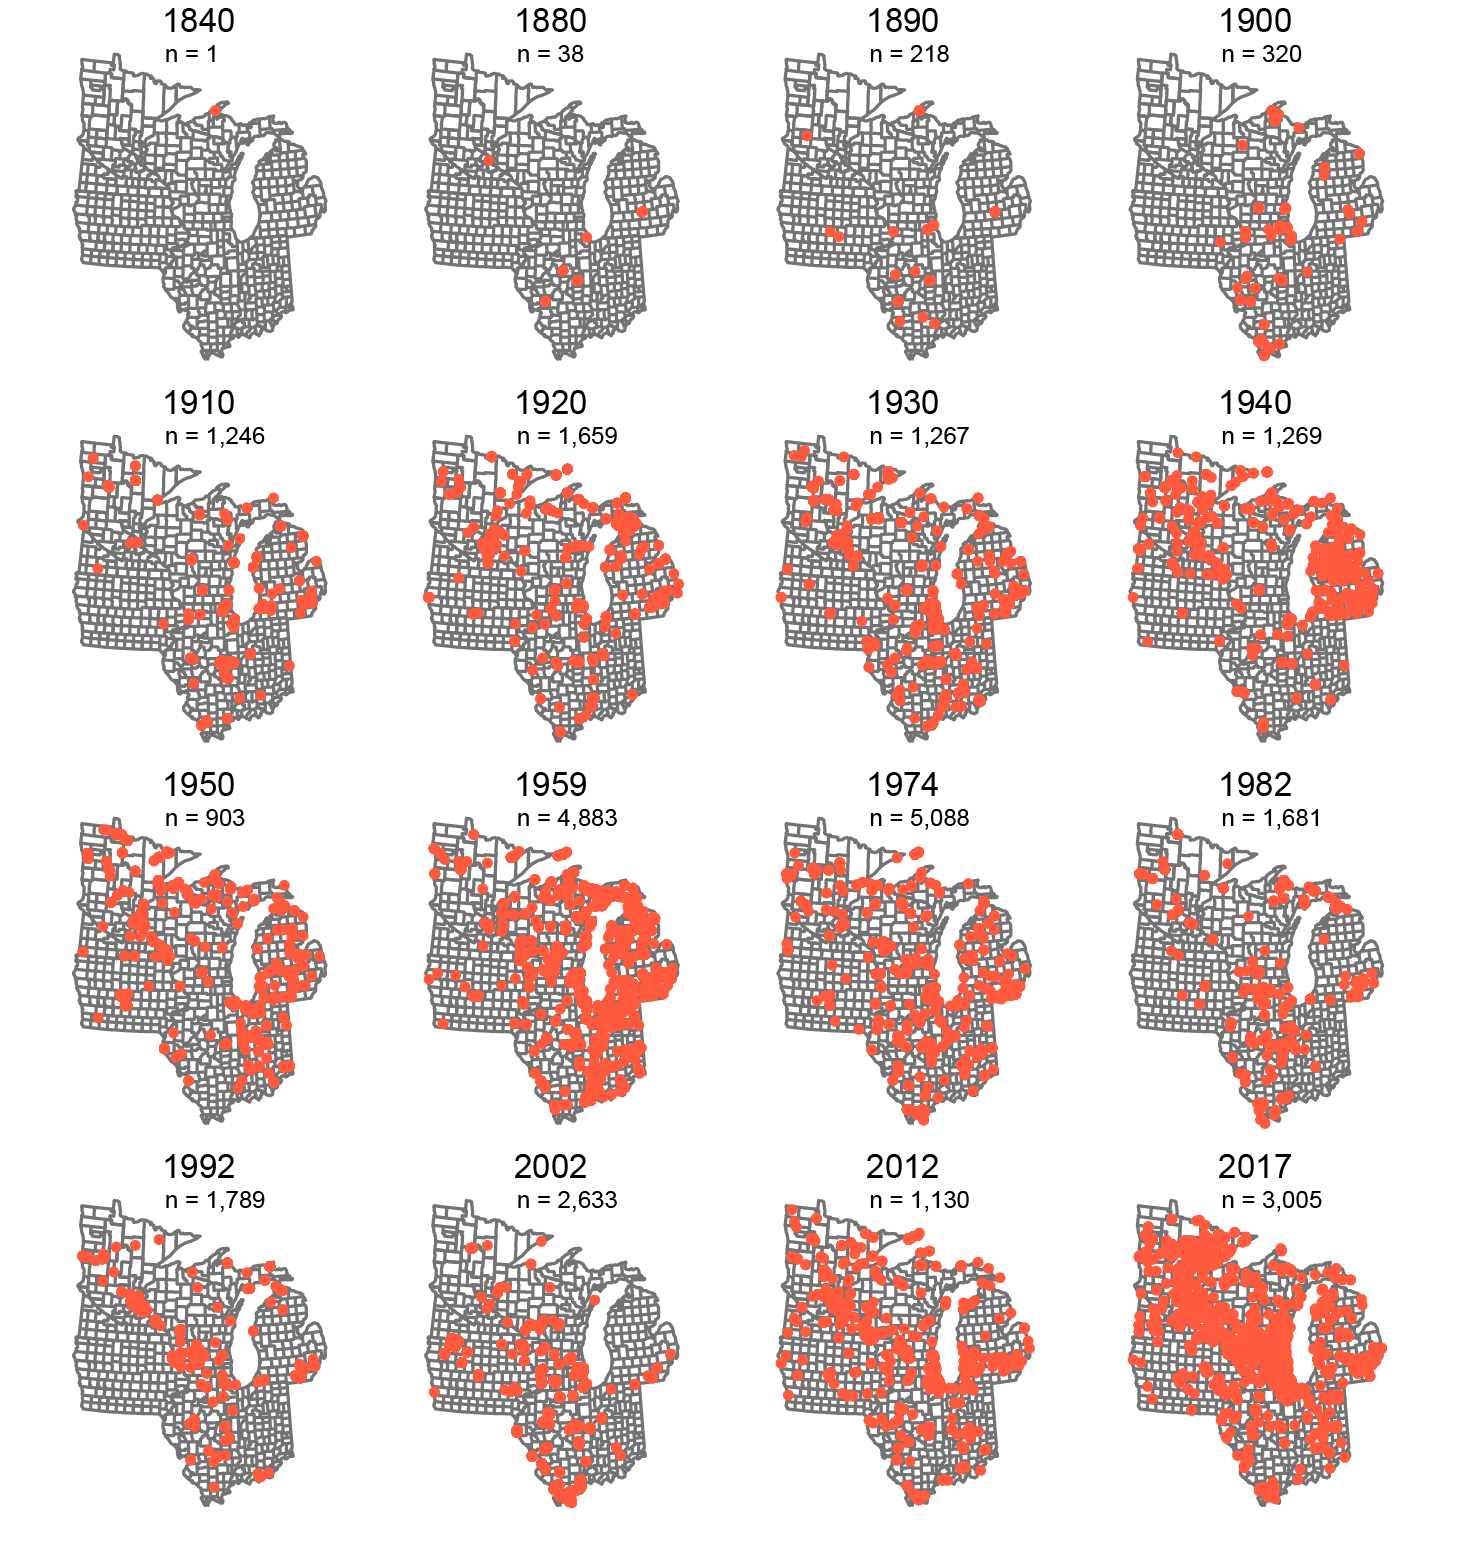
\includegraphics[width=0.6\textwidth,height=\textheight]{../ms_figs/fig_s3.png}

\textbf{Supplementary Figure 2:} Sample-based species accumulation
curves for each of 15 temporal bins (different colors) from which
estimated species richness was calculated (Fig. 1). Each accumulation
curve is constructed for temporal bins with a roughly equal number of
records. Solid lines are interpolated from data, while dashed lines are
extrapolated to a 6,000 record limit.

\clearpage

\newpage

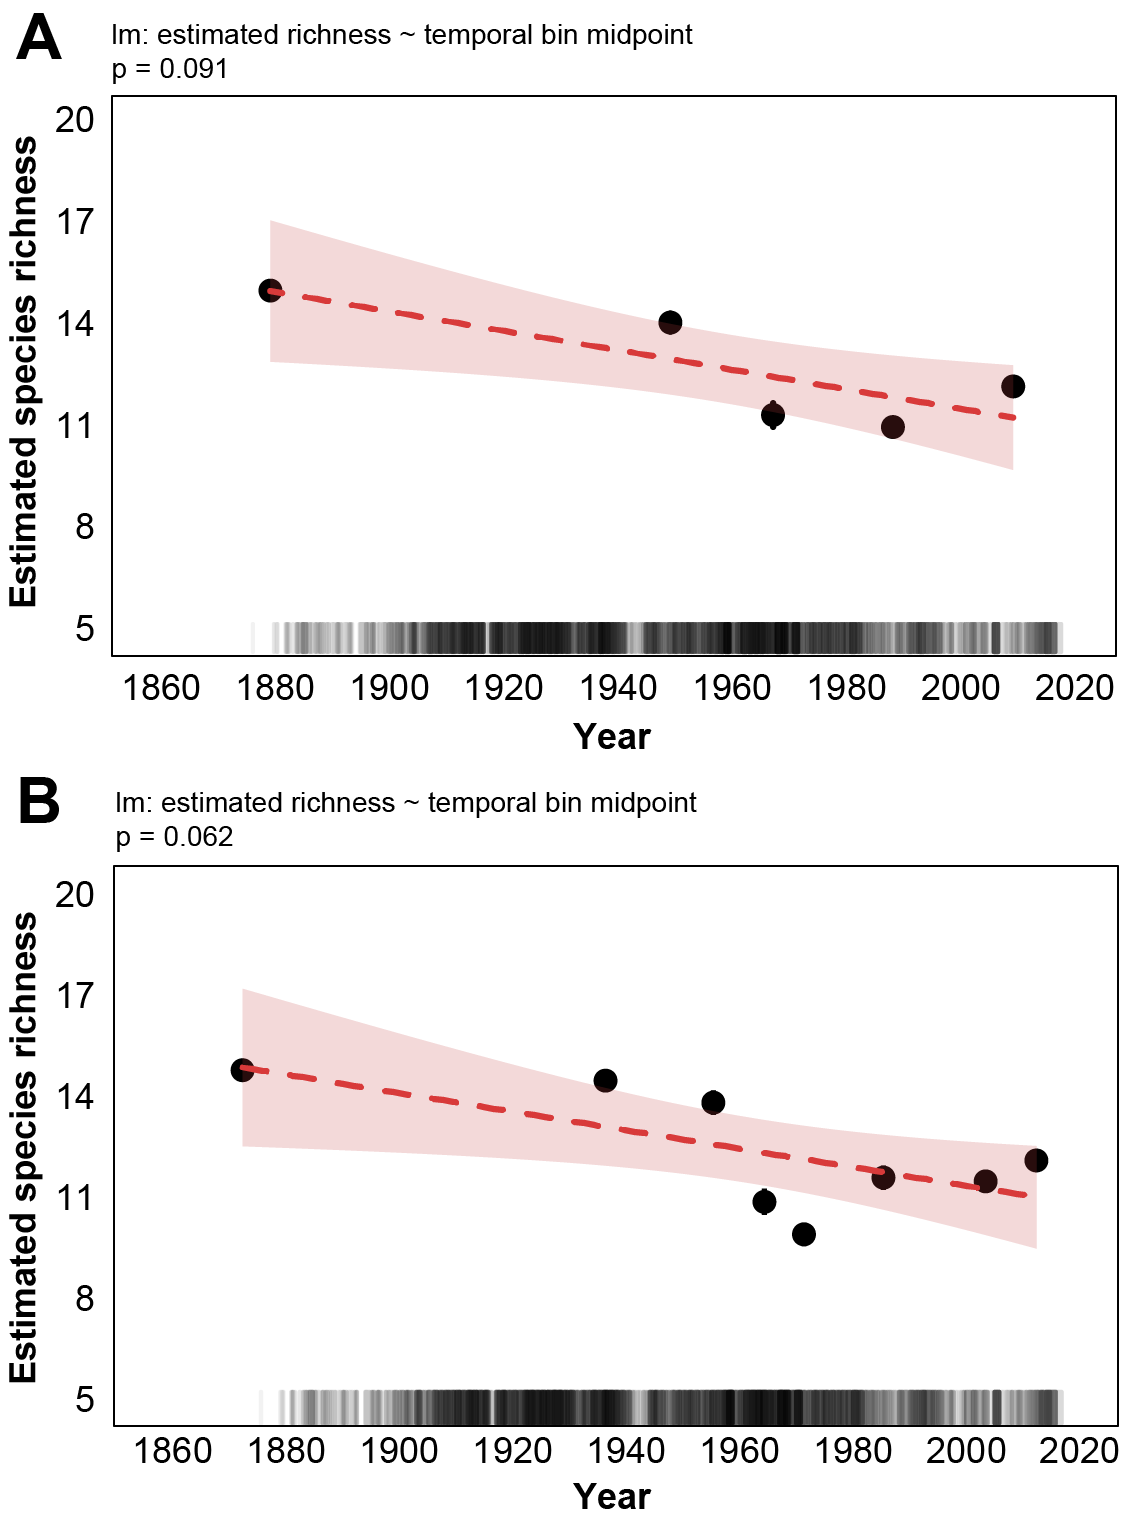
\includegraphics[width=0.6\textwidth,height=\textheight]{../ms_figs/fig_s1.png}

\textbf{Supplementary Figure 3:} Trend in rarified bumble bee species
richness from 1877-present for alternative numbers of temporal bins,
each representing approximately equal numbers of bumble bee records: (A)
5 temporal bins and (B) 8 temporal bins. Each point is plotted at the
midpoint of the temporal bin date range. Error bars are 95\% confidence
intervals. The fitted line is a linear model predicting estimated
species richness as a function of temporal bin order using the midpoint
year of the temporal bin as the predictor. Carpet plot represents
temporal collection year for all records from 1877 to present.

\clearpage

\newpage

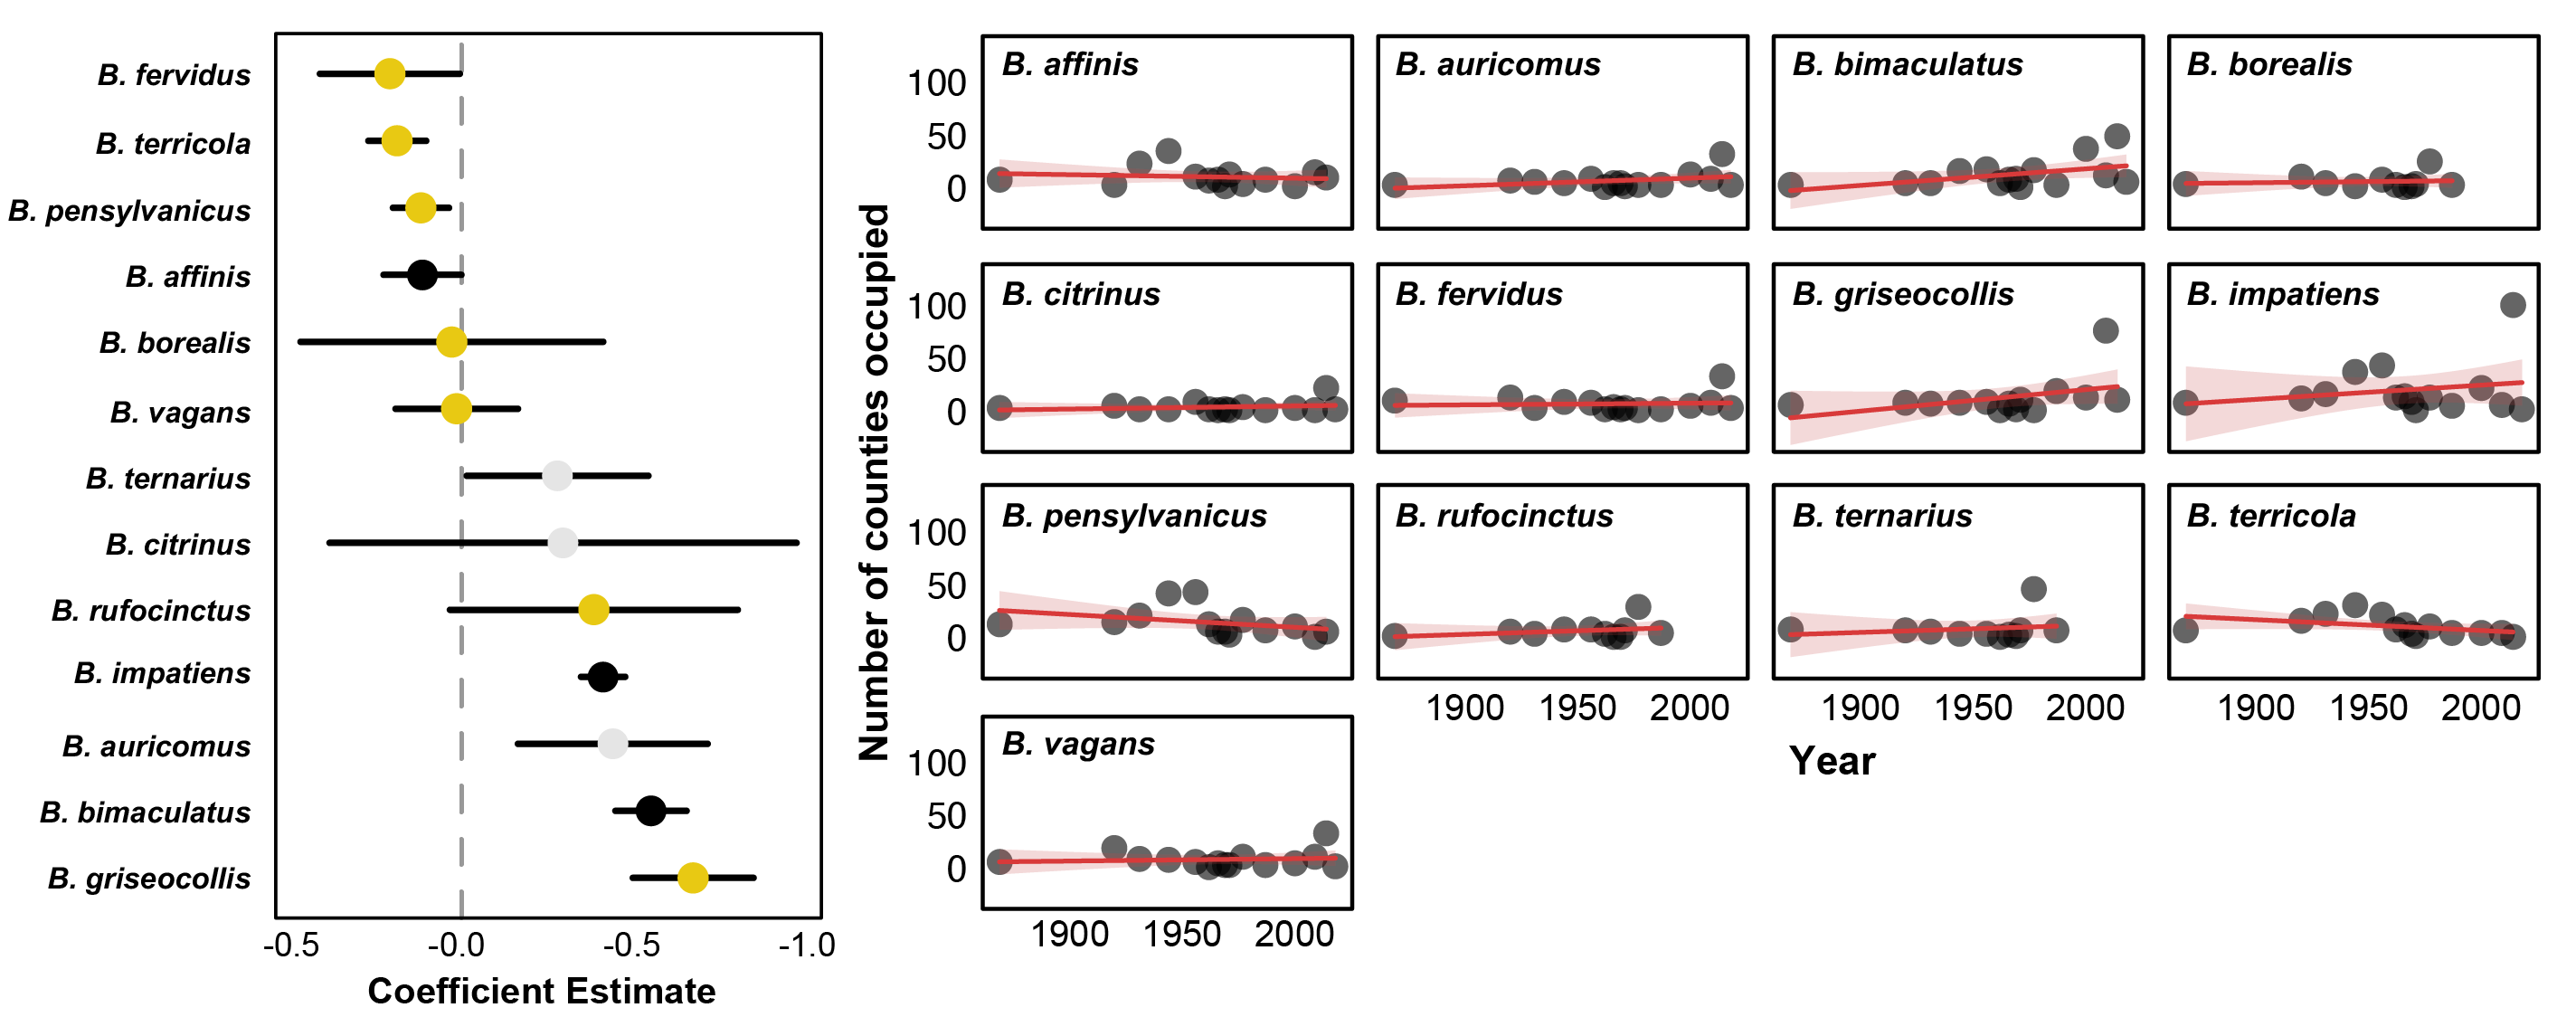
\includegraphics[width=1\textwidth,height=\textheight]{../ms_figs/fig6.png}

\textbf{Supplementary Figure 4:} (A) Fitted model coefficients for each
species for change in county occupancy over time. (B) For each species,
plotted temporal trends of county occupancy over time with fitted GLM
models with 95\% confidence interval. Point colors indicate species
relative abundance trend from 1870-present (see Fig. 3a): yellow points
denote species whose relative abundance declined, gray points denote no
change in relative abundance, and black points denote increases in
relative abundance.

\clearpage

\newpage

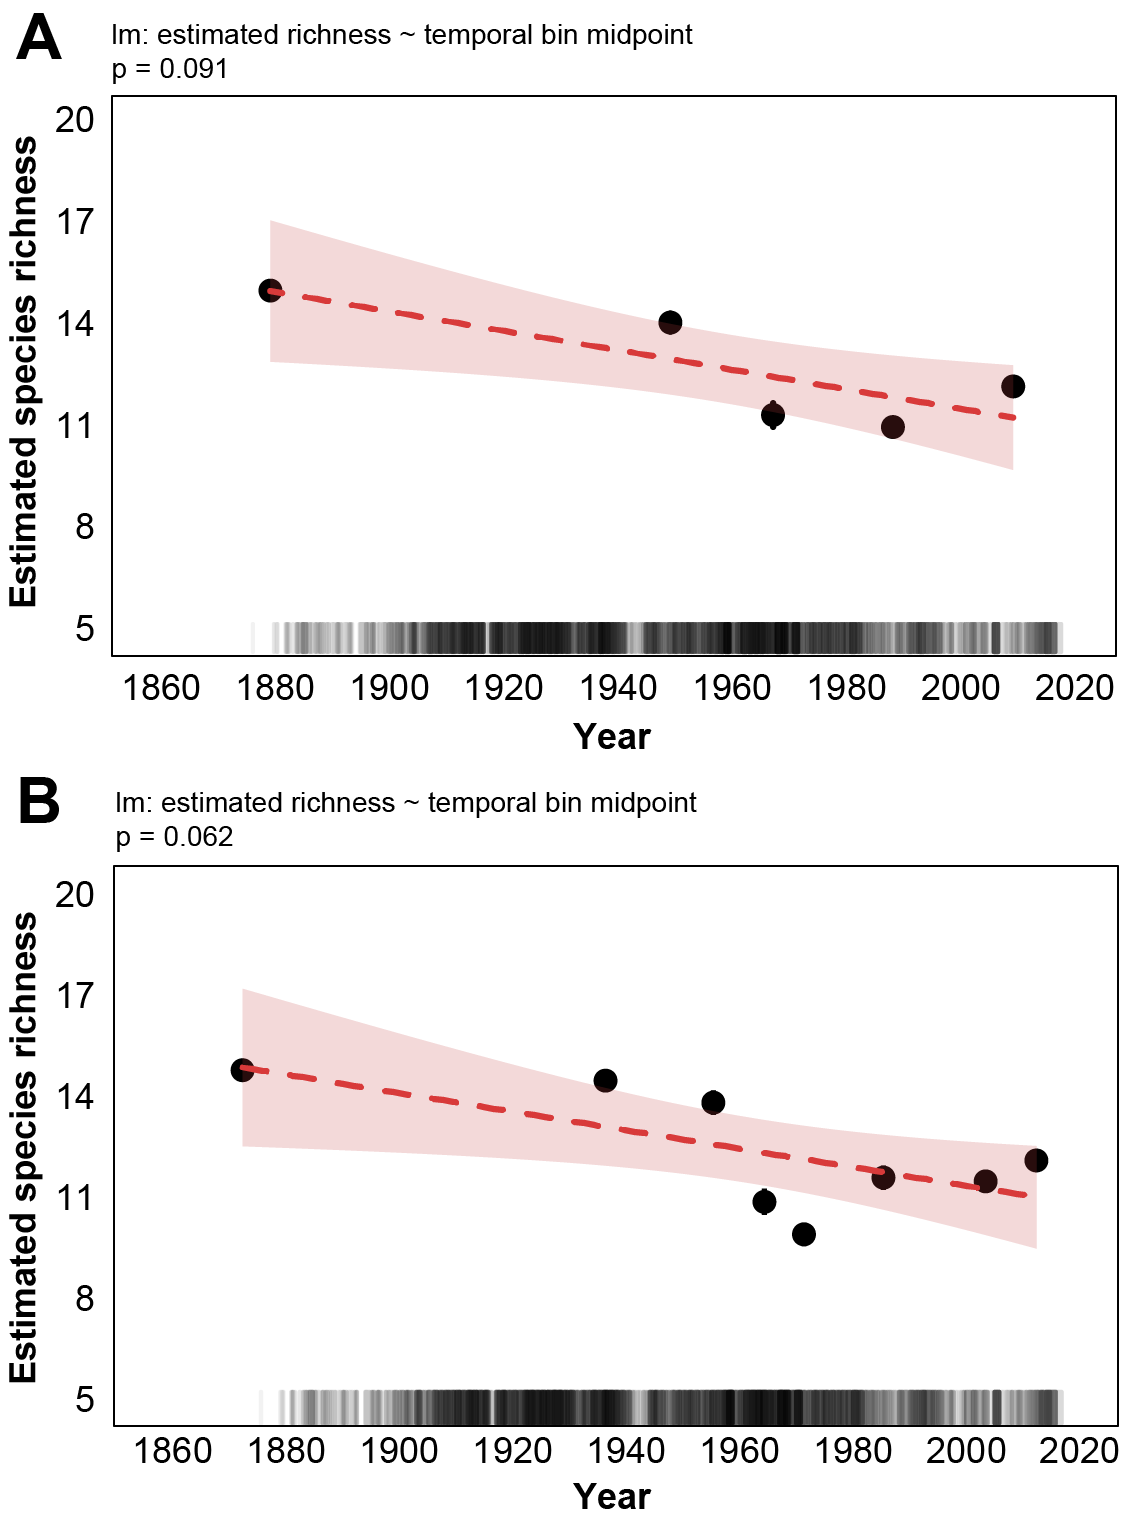
\includegraphics[width=1\textwidth,height=\textheight]{../ms_figs/fig_s4.png}

\textbf{Supplementary Figure 5:} Patterns of agricultural
intensification in two additional metrics from 1982-2012: (a) proportion
of county area in pasture and (c) proportion of county area treated with
insecticides. Color palettes derived using quantile binning. Inset
graphs (b,d) depict general trend of these two variables for each state
in the study area as modeled by a Loess curve. Values beneath years are
mean proportion ± SEM.

\clearpage

\newpage

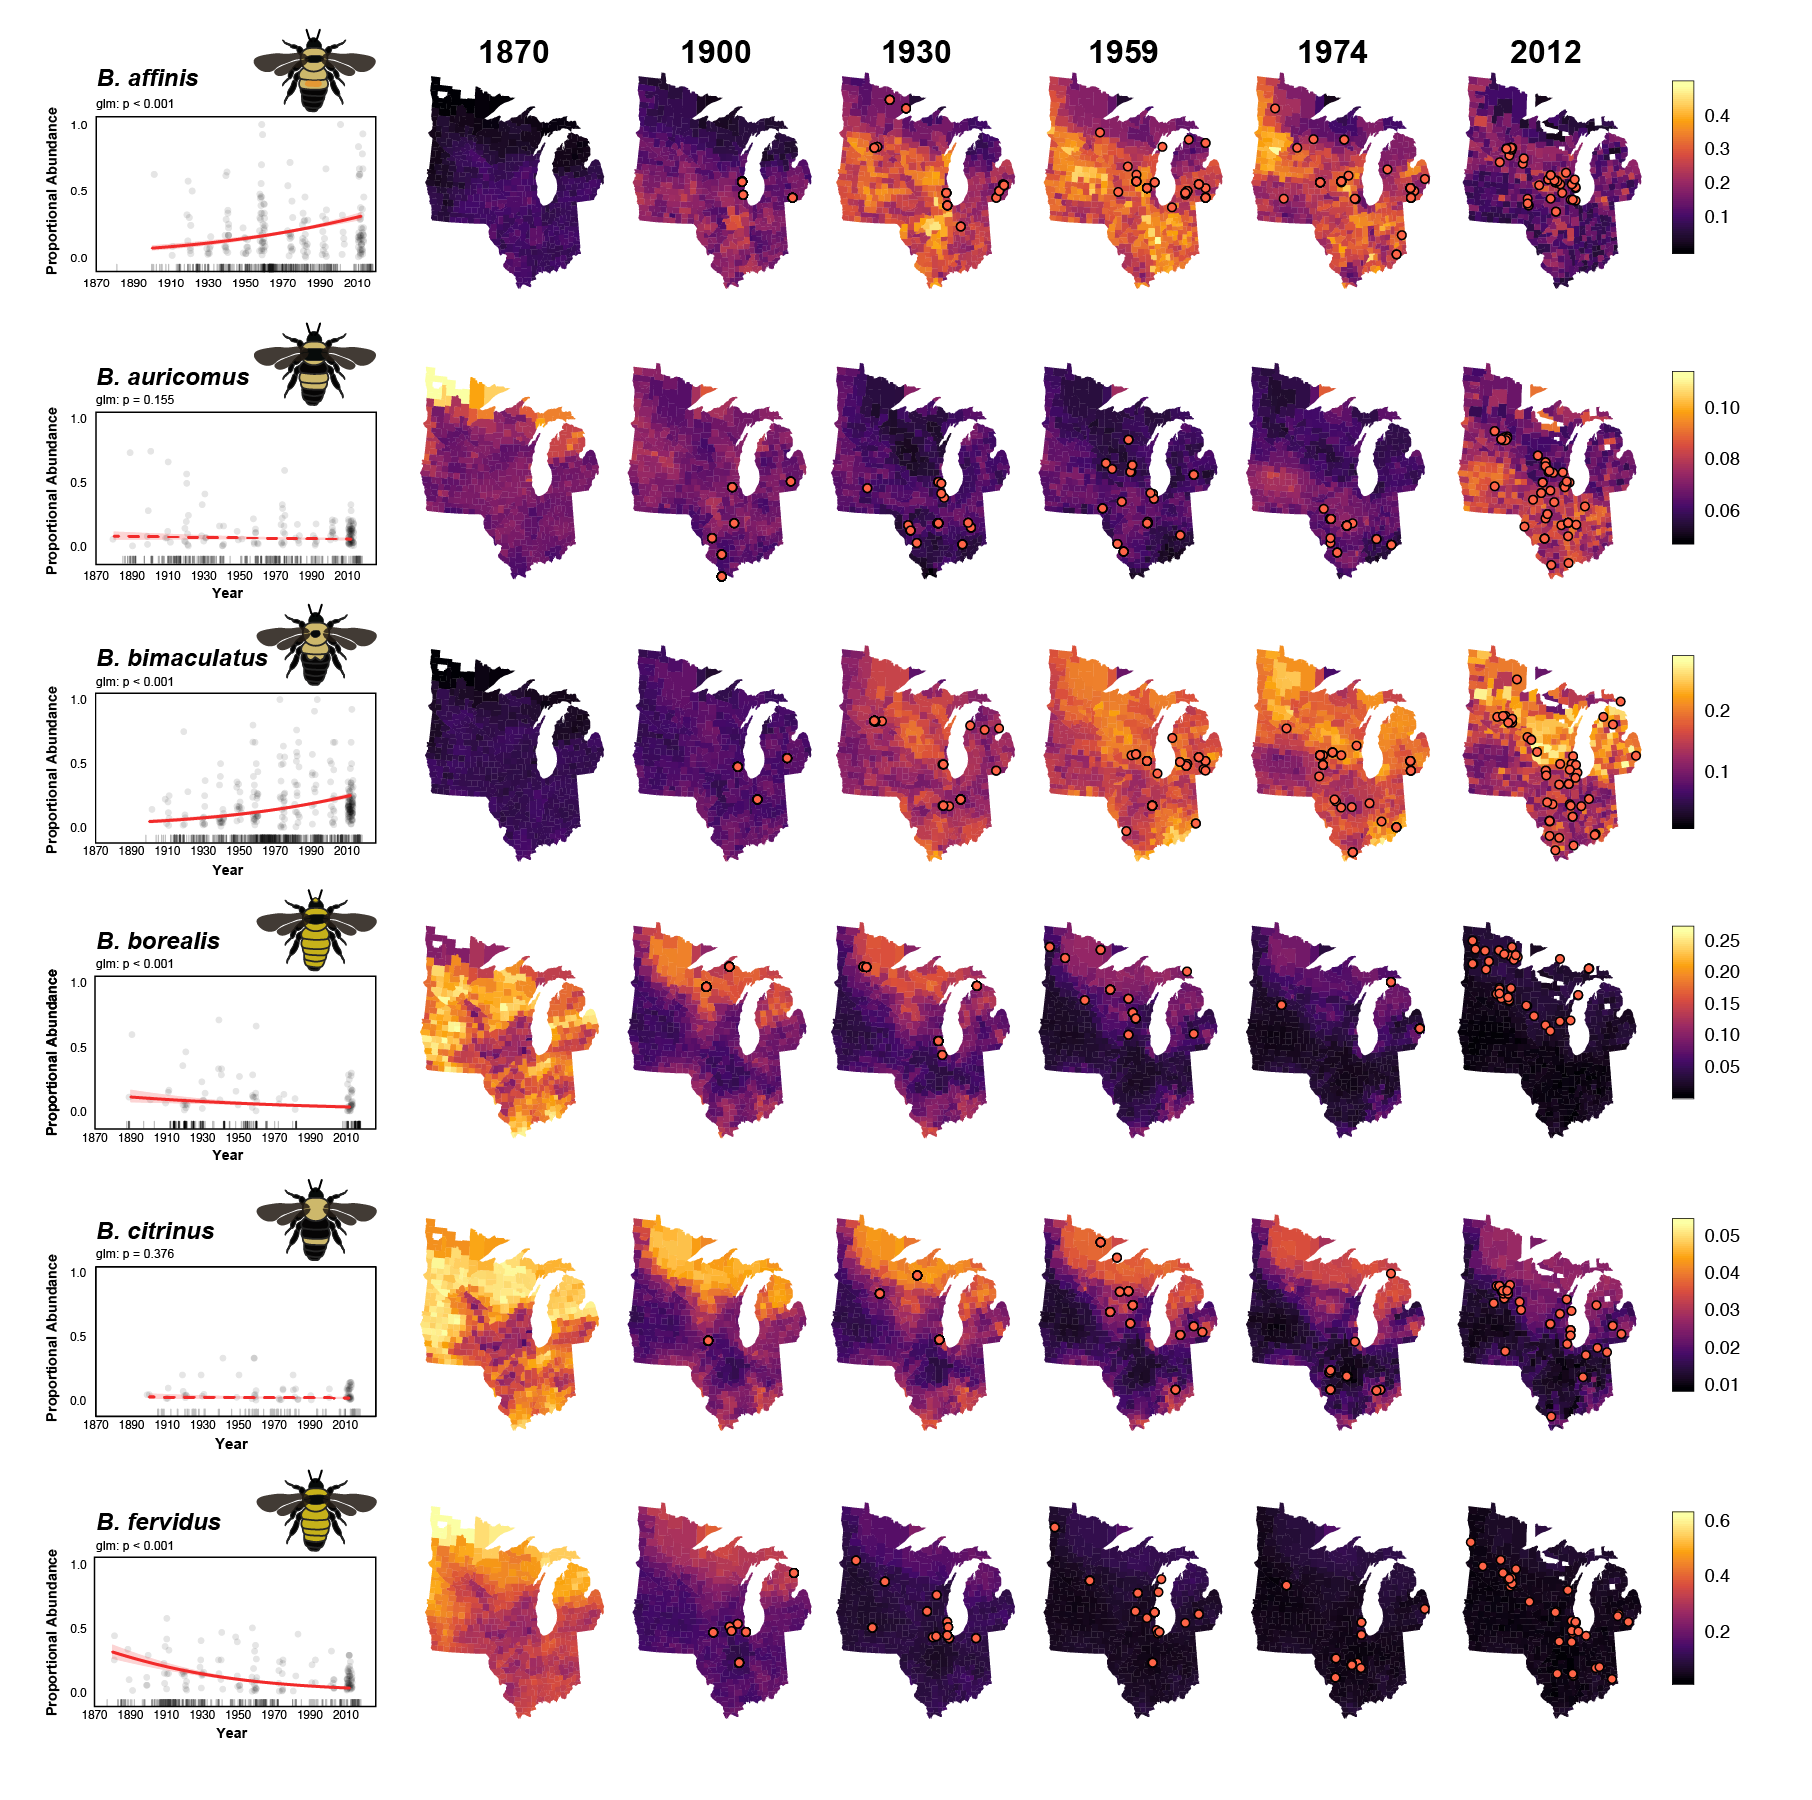
\includegraphics[width=1\textwidth,height=\textheight]{../ms_figs/fig4a.png}

\clearpage

\newpage

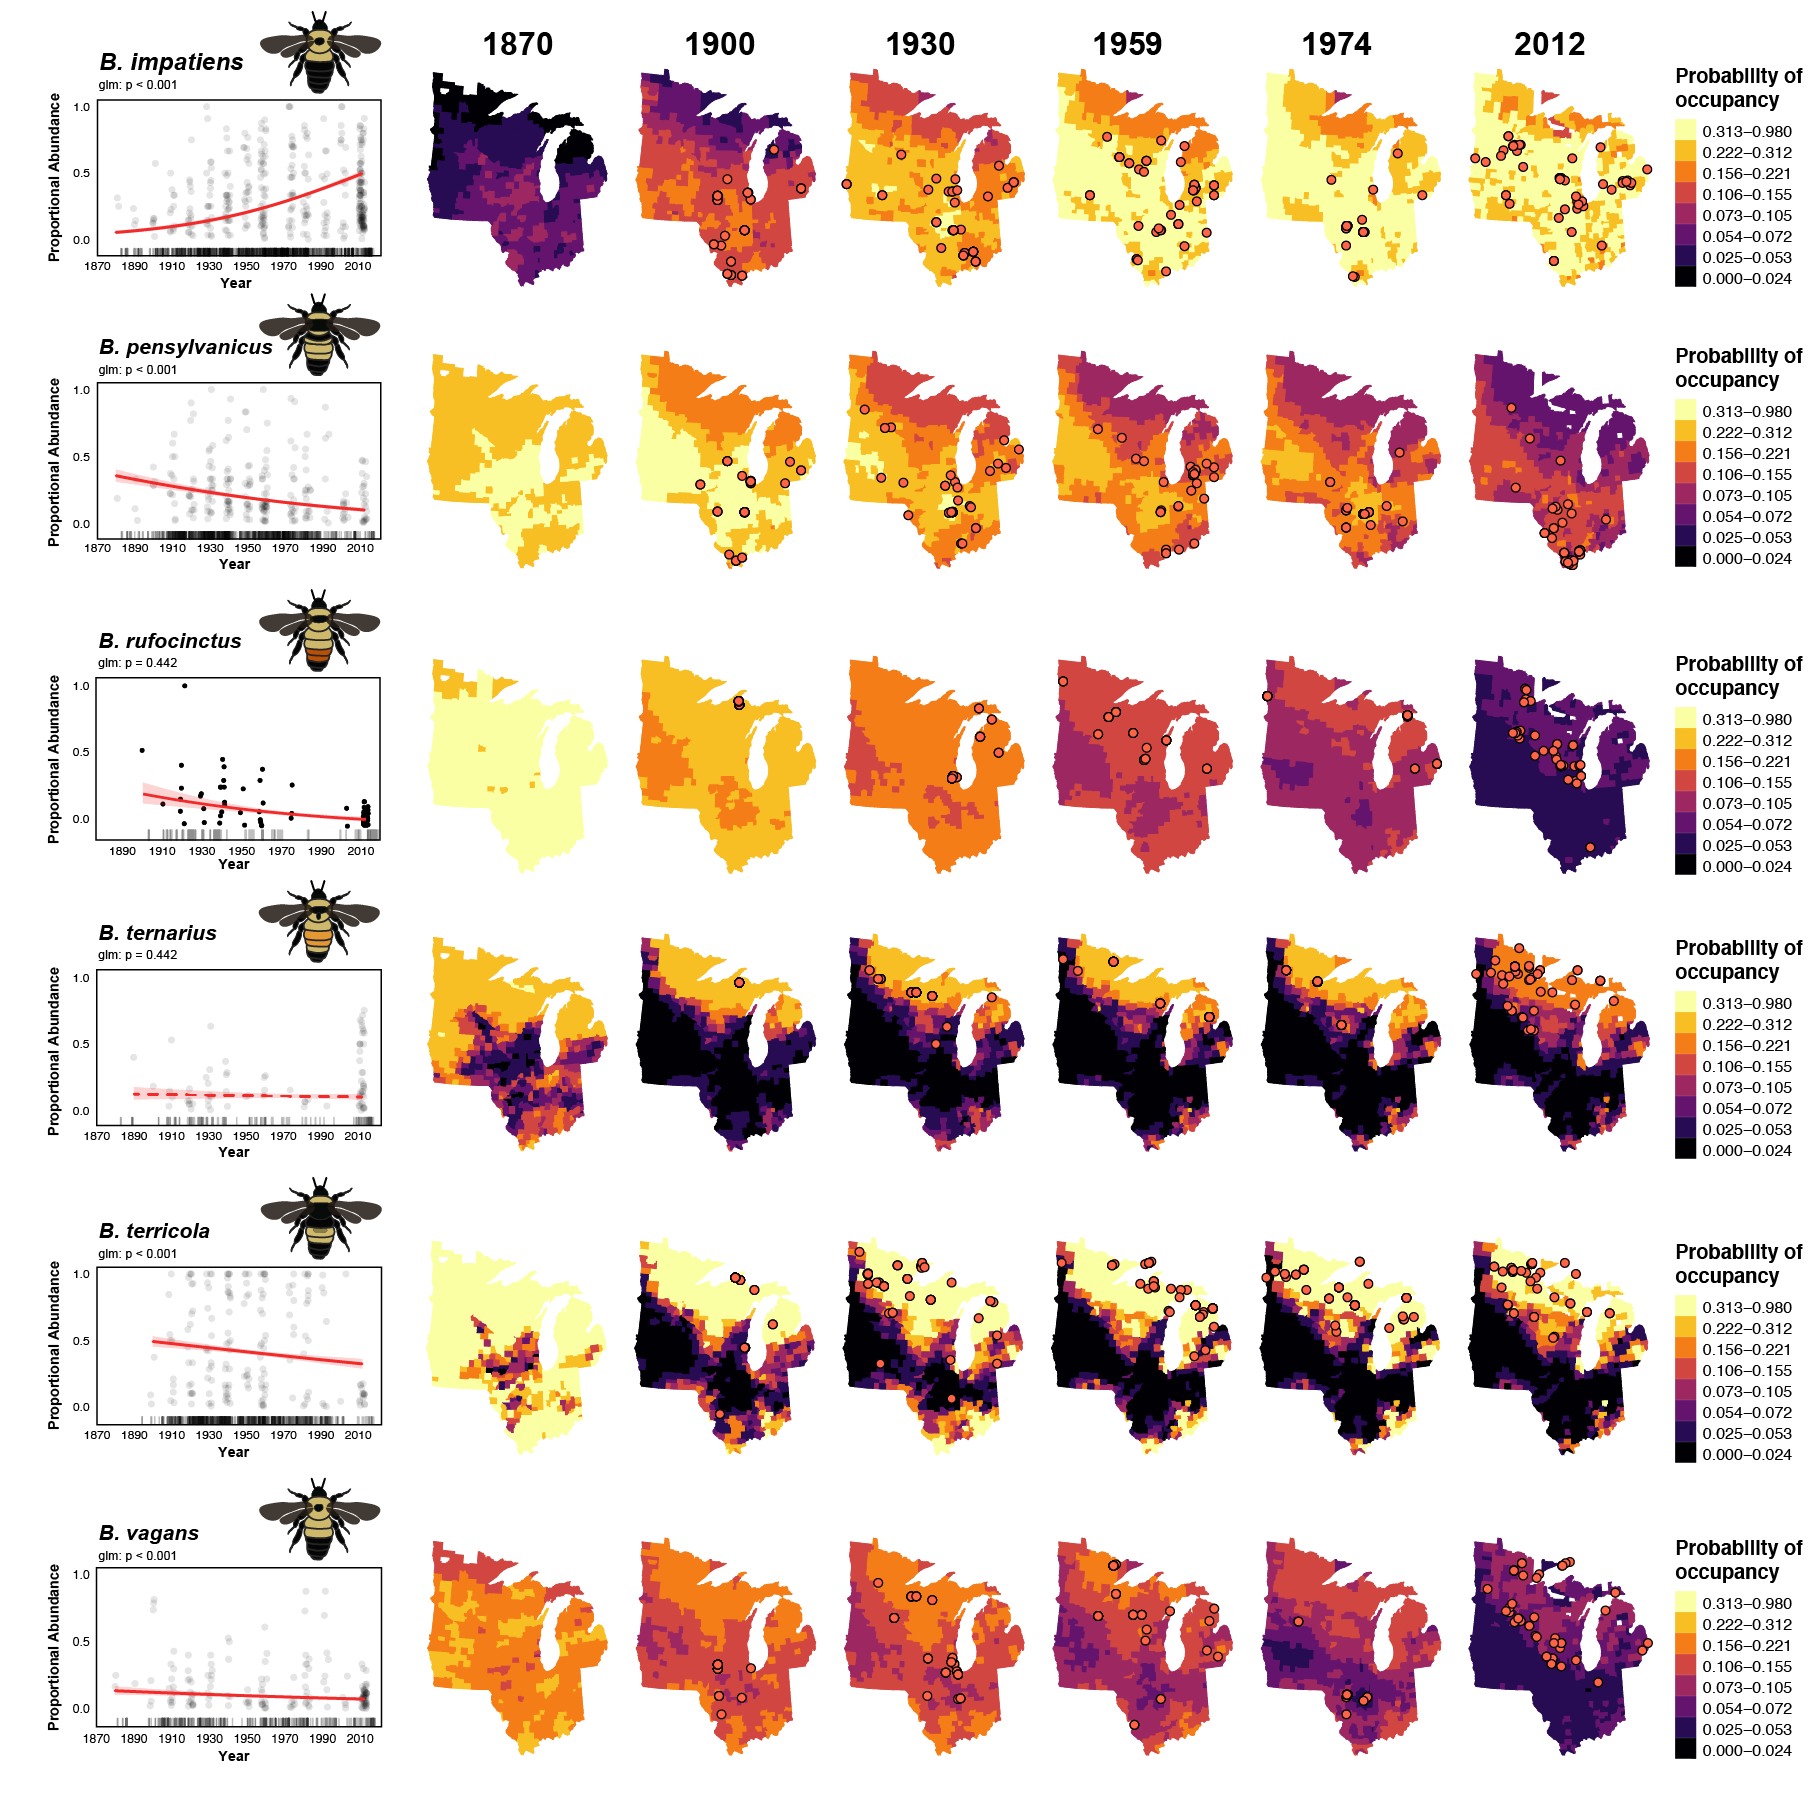
\includegraphics[width=1\textwidth,height=\textheight]{../ms_figs/fig4b.png}

\textbf{Supplementary Figure 6:} Fitted temporal trend of relative
abundance when modeled with agricultural intensity metrics along with
the predicted probability of occurrence for each study species in each
county given crop diversity and proportion cropland in each county.
Darker colors denote smaller probability of occurrence, while lighter
colors indicate larger probability of occurrence. Solid red lines denote
statistically clear trend in relative abundance over time (p \textless{}
0.05), while dashed lines denote statistically unclear trends (p
\textgreater{} 0.05). Points on temporal trend are slightly jittered for
visibility. Red points on each map are randomly selected occurrence
records with a maximum of 50 plotted per year.

\clearpage

\hypertarget{references}{%
\section*{References}\label{references}}
\addcontentsline{toc}{section}{References}

\hypertarget{refs}{}
\leavevmode\hypertarget{ref-Bartomeus2013}{}%
Bartomeus, Ignasi, Mia G. Park, Jason Gibbs, Bryan N. Danforth, Alan N.
Lakso, and Rachael Winfree. 2013. ``Biodiversity ensures
plant-pollinator phenological synchrony against climate change.''
\emph{Ecol. Lett.} 16 (11): 1331--8.
\url{https://doi.org/10.1111/ele.12170}.

\leavevmode\hypertarget{ref-Bartomeus2019}{}%
Bartomeus, I., J. R. Stavert, D. Ward, and O. Aguado. 2019. ``Historical
collections as a tool for assessing the global pollination crisis.''
\emph{Philos. Trans. R. Soc. B Biol. Sci.} 374 (1763): 1--9.
\url{https://doi.org/10.1098/rstb.2017.0389}.

\leavevmode\hypertarget{ref-Benton2002}{}%
Benton, Tim G., David M. Bryant, Lorna Cole, and Humphrey Q.P. Crick.
2002. ``Linking agricultural practice to insect and bird populations: A
historical study over three decades.'' \emph{J. Appl. Ecol.} 39 (4):
673--87. \url{https://doi.org/10.1046/j.1365-2664.2002.00745.x}.

\leavevmode\hypertarget{ref-Benton2003}{}%
Benton, Tim G., Juliet A. Vickery, and Jeremy D. Wilson. 2003.
``Farmland biodiversity: Is habitat heterogeneity the key?''
\emph{Trends Ecol. Evol.} 18 (4): 182--88.
\url{https://doi.org/10.1016/S0169-5347(03)00011-9}.

\leavevmode\hypertarget{ref-Biesmeijer2006}{}%
Biesmeijer, J. C. 2006. ``Parallel Declines in Pollinators and
Insect-Pollinated Plants in Britain and the Netherlands.'' \emph{Science
(80-. ).} 313 (5785): 351--54.
\url{https://doi.org/10.1126/science.1127863}.

\leavevmode\hypertarget{ref-Brown2011}{}%
Brown, Paul W., and Lisa A. Schulte. 2011. ``Agricultural landscape
change (1937-2002) in three townships in Iowa, USA.'' \emph{Landsc.
Urban Plan.} 100 (3): 202--12.
\url{https://doi.org/10.1016/j.landurbplan.2010.12.007}.

\leavevmode\hypertarget{ref-Cameron2011}{}%
Cameron, Sydney A, Jeffrey D Lozier, James P Strange, Jonathan B Koch,
Nils Cordes, Leellen F Solter, Terry L Griswold, and Gene E Robinson.
2011. ``Patterns of widespread decline in North American bumble bees.''
\emph{Proc. Natl. Acad. Sci. U. S. A.} 108 (2): 662--67.
\url{https://doi.org/10.1073/pnas.1014743108}.

\leavevmode\hypertarget{ref-Carvell2006b}{}%
Carvell, Claire, David B. Roy, Simon M. Smart, Richard F. Pywell, Chris
D. Preston, and Dave Goulson. 2006. ``Declines in forage availability
for bumblebees at a national scale.'' \emph{Biol. Conserv.} 132 (4):
481--89. \url{https://doi.org/10.1016/j.biocon.2006.05.008}.

\leavevmode\hypertarget{ref-Colla2012}{}%
Colla, Sheila R., Fawziah Gadallah, Leif Richardson, David Wagner, and
Lawrence Gall. 2012. ``Assessing declines of North American bumble bees
(Bombus spp.) using museum specimens.'' \emph{Biodivers. Conserv.} 21
(14): 3585--95. \url{https://doi.org/10.1007/s10531-012-0383-2}.

\leavevmode\hypertarget{ref-Colla2008}{}%
Colla, Sheila R., and Laurence Packer. 2008. ``Evidence for decline in
eastern North American bumblebees (Hymenoptera: Apidae), with special
focus on Bombus affinis Cresson.'' \emph{Biodivers. Conserv.}
\url{https://doi.org/10.1007/s10531-008-9340-5}.

\leavevmode\hypertarget{ref-Crone2016}{}%
Crone, Elizabeth E., Neal M. Williams, and Ecology Letters. 2016.
``Bumble bee colony dynamics: Quantifying the importance of land use and
floral resources for colony growth and queen production.'' Edited by
Rebecca Irwin. \emph{Ecol. Lett.} 19 (4): 460--68.
\url{https://doi.org/10.1111/ele.12581}.

\leavevmode\hypertarget{ref-Fahrig2011b}{}%
Fahrig, Lenore, Jacques Baudry, Lluís Brotons, Françoise G Burel, Thomas
O Crist, Robert J Fuller, Clelia Sirami, Gavin M Siriwardena, and
Jean-Louis Martin. 2011. ``Functional landscape heterogeneity and animal
biodiversity in agricultural landscapes.'' \emph{Ecol. Lett.} 14 (2):
101--12. \url{https://doi.org/10.1111/j.1461-0248.2010.01559.x}.

\leavevmode\hypertarget{ref-Foley2005a}{}%
Foley, Jonathan A., Ruth DeFries, Gregory P. Asner, Carol Barford,
Gordon Bonan, Stephen R. Carpenter, F. Stuart Chapin, et al. 2005.
``Global consequences of land use.'' \emph{Science (80-. ).} 309 (5734):
570--74. \url{https://doi.org/10.1126/science.1111772}.

\leavevmode\hypertarget{ref-Foley2011b}{}%
Foley, Jonathan A., Navin Ramankutty, Kate A. Brauman, Emily S. Cassidy,
James S. Gerber, Matt Johnston, Nathaniel D. Mueller, et al. 2011.
``Solutions for a cultivated planet.'' \emph{Nature} 478 (7369):
337--42. \url{https://doi.org/10.1038/nature10452}.

\leavevmode\hypertarget{ref-Grixti2009}{}%
Grixti, Jennifer C., Lisa T. Wong, Sydney a. Cameron, and Colin Favret.
2009. ``Decline of bumble bees (Bombus) in the North American Midwest.''
\emph{Biol. Conserv.} 142 (1): 75--84.
\url{https://doi.org/10.1016/j.biocon.2008.09.027}.

\leavevmode\hypertarget{ref-Hallmann2017}{}%
Hallmann, Caspar A., Martin Sorg, Eelke Jongejans, Henk Siepel, Nick
Hofland, Heinz Schwan, Werner Stenmans, et al. 2017. ``More than 75
percent decline over 27 years in total flying insect biomass in
protected areas.'' \emph{PLoS One} 12 (10): e0185809.
\url{https://doi.org/10.1371/journal.pone.0185809}.

\leavevmode\hypertarget{ref-Hass2018a}{}%
Hass, Annika Louise, Lara Brachmann, Péter Batáry, Yann Clough, Hermann
Behling, and Teja Tscharntke. 2018. ``Maize-dominated landscapes reduce
bumblebee colony growth through pollen diversity loss.'' \emph{J. Appl.
Ecol.}, no. September: 1--11.
\url{https://doi.org/10.1111/1365-2664.13296}.

\leavevmode\hypertarget{ref-Hsieh2016}{}%
Hsieh, T. C., K. H. Ma, and Anne Chao. 2016. ``iNEXT: an R package for
rarefaction and extrapolation of species diversity (Hill numbers).''
\emph{Methods Ecol. Evol.} 7 (12): 1451--6.
\url{https://doi.org/10.1111/2041-210X.12613}.

\leavevmode\hypertarget{ref-Jacobson2018a}{}%
Jacobson, Molly M., Erika M. Tucker, Minna E. Mathiasson, and Sandra M.
Rehan. 2018. ``Decline of bumble bees in northeastern North America,
with special focus on Bombus terricola.'' \emph{Biol. Conserv.} 217
(August 2017): 437--45.
\url{https://doi.org/10.1016/j.biocon.2017.11.026}.

\leavevmode\hypertarget{ref-Kerr2015}{}%
Kerr, Jeremy T, Alana Pindar, Paul Galpern, Laurence Packer, Simon G
Potts, Stuart M Roberts, Pierre Rasmont, et al. 2015. ``Climate change
impacts on bumblebees converge across continents.'' \emph{Science (80-.
).} 349 (6244): 177--80. \url{https://doi.org/10.1126/science.aaa7031}.

\leavevmode\hypertarget{ref-Kleijn2008}{}%
Kleijn, David, and Ivo Raemakers. 2008. ``A retrospective analysis of
pollen host plant use by stable and declining bumble bee species.''
\emph{Ecology} 89 (7): 1811--23.
\url{https://doi.org/10.1890/07-1275.1}.

\leavevmode\hypertarget{ref-Klein2007g}{}%
Klein, Alexandra-Maria, Bernard E Vaissière, James H Cane, Ingolf
Steffan-Dewenter, Saul a Cunningham, Claire Kremen, and Teja Tscharntke.
2007. ``Importance of pollinators in changing landscapes for world
crops.'' \emph{Proc. Biol. Sci.} 274 (1608): 303--13.
\url{https://doi.org/10.1098/rspb.2006.3721}.

\leavevmode\hypertarget{ref-Meehan2015}{}%
Meehan, Timothy D., and Claudio Gratton. 2015. ``A consistent positive
association between landscape simplification and insecticide use across
the Midwestern US from 1997 through 2012.'' \emph{Environ. Res. Lett.}
10 (11). \url{https://doi.org/10.1088/1748-9326/10/11/114001}.

\leavevmode\hypertarget{ref-Meehan2010a}{}%
Meehan, Timothy D, Allen H Hurlbert, and Claudio Gratton. 2010. ``Bird
communities in future bioenergy landscapes of the Upper Midwest.''
\emph{Proc. Natl. Acad. Sci. U. S. A.} 107 (43): 18533--8.
\url{https://doi.org/10.1073/pnas.1008475107}.

\leavevmode\hypertarget{ref-Meehan2011}{}%
Meehan, Timothy D, Ben P Werling, Douglas a Landis, and Claudio Gratton.
2011. ``Agricultural landscape simplification and insecticide use in the
Midwestern United States.'' \emph{Proc. Natl. Acad. Sci. U. S. A.} 108
(28): 11500--11505. \url{https://doi.org/10.1073/pnas.1100751108}.

\leavevmode\hypertarget{ref-Morales2013}{}%
Morales, Carolina L., Marina P. Arbetman, Sydney A. Cameron, and Marcelo
A. Aizen. 2013. ``Rapid ecological replacement of a native bumble bee by
invasive species.'' \emph{Front. Ecol. Environ.} 11 (10): 529--34.
\url{https://doi.org/10.1890/120321}.

\leavevmode\hypertarget{ref-Pearce2006}{}%
Pearce, Jennie L., and Mark S. Boyce. 2006. ``Modelling distribution and
abundance with presence-only data.'' \emph{J. Appl. Ecol.} 43 (3):
405--12. \url{https://doi.org/10.1111/j.1365-2664.2005.01112.x}.

\leavevmode\hypertarget{ref-Rhemtulla2007a}{}%
Rhemtulla, Jeanine M., David J. Mladenoff, and Murray K. Clayton. 2007.
``Regional land-cover conversion in the U.S. upper Midwest: Magnitude of
change and limited recovery (1850-1935-1993).'' \emph{Landsc. Ecol.} 22
(SUPPL. 1): 57--75. \url{https://doi.org/10.1007/s10980-007-9117-3}.

\leavevmode\hypertarget{ref-Richardson2018}{}%
Richardson, L.L, K.P McFarland, S Zahendra, and S Hardy. 2018. ``Bumble
bee (\textless{}i\textgreater{}Bombus\textless{}/i\textgreater{})
distribution and diversity in Vermont, USA: A century of change.''
\emph{J. Insect Conserv.} In Review (0): 0.
\url{https://doi.org/10.1007/s10841-018-0113-5}.

\leavevmode\hypertarget{ref-Robinson2002}{}%
Robinson, Robert A., and William J. Sutherland. 2002. ``Post-war changes
in arable farming and biodiversity in Great Britain.'' \emph{J. Appl.
Ecol.} 39 (1): 157--76.
\url{https://doi.org/10.1046/j.1365-2664.2002.00695.x}.

\leavevmode\hypertarget{ref-Schellhorn2015c}{}%
Schellhorn, Nancy A., Vesna Gagic, and Riccardo Bommarco. 2015. ``Time
will tell: Resource continuity bolsters ecosystem services.''
\emph{Trends Ecol. Evol.} 30 (9): 524--30.
\url{https://doi.org/10.1016/j.tree.2015.06.007}.

\leavevmode\hypertarget{ref-Scheper2014}{}%
Scheper, Jeroen, Menno Reemer, Ruud van Kats, Wim A. Ozinga, Giel T. J.
van der Linden, Joop H. J. Schaminée, Henk Siepel, and David Kleijn.
2014. ``Museum specimens reveal loss of pollen host plants as key factor
driving wild bee decline in The Netherlands.'' \emph{Proc. Natl. Acad.
Sci.} 111 (49): 201412973.
\url{https://doi.org/10.1073/pnas.1412973111}.

\leavevmode\hypertarget{ref-Schmid-Hempel1998a}{}%
Schmid-Hempel, Regula, and Paul Schmid-Hempel. 1998. ``Colony
performance and immunocompetence of a social insect, Bombus terrestris,
in poor and variable environments.'' \emph{Funct. Ecol.} 12 (1): 22--30.
\url{https://doi.org/10.1046/j.1365-2435.1998.00153.x}.

\leavevmode\hypertarget{ref-Seibold2019}{}%
Seibold, Sebastian, Martin M Gossner, Nadja K Simons, Nico Blüthgen,
Didem Ambarl, Christian Ammer, Jürgen Bauhus, et al. 2019. ``Arthropod
decline in grasslands and forests is associated with drivers at
landscape level.'' \emph{Nature} 574 (February): 1--34.
\url{https://doi.org/10.1038/s41586-019-1684-3}.

\leavevmode\hypertarget{ref-Sirami2019}{}%
Sirami, Clélia, Nicolas Gross, Aliette Bosem Baillod, Colette Bertrand,
Romain Carrié, Annika Hass, Laura Henckel, et al. 2019. ``Increasing
crop heterogeneity enhances multitrophic diversity across agricultural
regions.'' \emph{Proc. Natl. Acad. Sci.} 116 (33): 201906419.
\url{https://doi.org/10.1073/pnas.1906419116}.

\leavevmode\hypertarget{ref-Smith1998}{}%
Smith, Daryl D. 1998. ``Iowa prairie: Original extent and loss,
preservation and recovery attempts.'' \emph{J. Iowa Acad. Sci.} 105 (3):
94--108.

\leavevmode\hypertarget{ref-Soroye2020}{}%
Soroye, Peter, Tim Newbold, and Jeremy Kerr. 2020. ``Climate change
contributes to widespread declines among bumble bees across
continents.'' \emph{Science (80-. ).} 367 (6478): 685--88.
\url{https://doi.org/10.1126/science.aax8591}.

\leavevmode\hypertarget{ref-Steffan-Dewenter2005c}{}%
Steffan-Dewenter, Ingolf, Simon G. Potts, Laurence Packer, and Jaboury
Ghazoul. 2005. ``Pollinator diversity and crop pollination services are
at risk {[}3{]} (multiple letters).'' \emph{Trends Ecol. Evol.} 20 (12):
651--53. \url{https://doi.org/10.1016/j.tree.2005.09.004}.

\leavevmode\hypertarget{ref-Tilman2011}{}%
Tilman, David, Christian Balzer, Jason Hill, and Belinda L. Befort.
2011. ``Global food demand and the sustainable intensification of
agriculture.'' \emph{Proc. Natl. Acad. Sci. U. S. A.} 108 (50):
20260--4. \url{https://doi.org/10.1073/pnas.1116437108}.

\leavevmode\hypertarget{ref-Tscharntke2012}{}%
Tscharntke, Teja, Yann Clough, Thomas C. Wanger, Louise Jackson, Iris
Motzke, Ivette Perfecto, John Vandermeer, and Anthony Whitbread. 2012.
``Global food security, biodiversity conservation and the future of
agricultural intensification.'' \emph{Biol. Conserv.} 151 (1): 53--59.
\url{https://doi.org/10.1016/j.biocon.2012.01.068}.

\leavevmode\hypertarget{ref-Tylianakis2013a}{}%
Tylianakis, Jason M. 2013. ``The global plight of pollinators.''
\emph{Science (80-. ).} 339 (6127): 1532--3.
\url{https://doi.org/10.1126/science.1235464}.

\leavevmode\hypertarget{ref-Vaudo2015}{}%
Vaudo, Anthony D., John F. Tooker, Christina M. Grozinger, and Harland
M. Patch. 2015. ``Bee nutrition and floral resource restoration.''
\emph{Curr. Opin. Insect Sci.} 10: 133--41.
\url{https://doi.org/10.1016/j.cois.2015.05.008}.

\leavevmode\hypertarget{ref-Westphal2009a}{}%
Westphal, C., I. Steffan-Dewenter, and T. Tscharntke. 2009. ``Mass
flowering oilseed rape improves early colony growth but not sexual
reproduction of b1. Westphal, C., Steffan-Dewenter, I. \& Tscharntke, T.
(2009). Mass flowering oilseed rape improves early colony growth but not
sexual reproduction of bumblebees. J.'' \emph{J. Appl. Ecol.} 46 (1):
187--93. \url{https://doi.org/10.1111/j.1365-2664.2008.01580.x}.

\leavevmode\hypertarget{ref-Williams2012b}{}%
Williams, Neal M., James Regetz, and Claire Kremen. 2012.
``Landscape-scale resources promote colony growth but not reproductive
performance of bumble bees.'' \emph{Ecology} 93 (5): 1049--58.
\url{https://doi.org/10.1890/11-1006.1}.

\leavevmode\hypertarget{ref-Wood2019}{}%
Wood, Thomas J., Jason Gibbs, Kelsey K. Graham, and Rufus Isaacs. 2019.
``Narrow pollen diets are associated with declining Midwestern bumble
bee species.'' \emph{Ecology} 0 (0).
\url{https://doi.org/10.1002/ecy.2697}.


\end{document}
